\documentclass[1p,preprint,fleqn,number,sort&compress,times]{elsarticle}

\usepackage{amsmath}
\usepackage{amssymb}
\usepackage{booktabs}
\usepackage{calc}
\usepackage{color}
\usepackage{enumitem}
\usepackage{esvect}
\usepackage{fmtcount}
\usepackage{ifthen}
\usepackage{pgfplots}
\usepackage{pifont}
\usepackage{siunitx}
\usepackage{stackengine}
\usepackage{subcaption}
\usepackage{tikz}
\usepackage{xfrac}
\usepackage{xspace}

\usepackage{accents}
\usepackage[colorlinks]{hyperref}

\def\stackalignment{l}
\usetikzlibrary{arrows.meta}
\usetikzlibrary{calc}
\usetikzlibrary{decorations.pathmorphing}
\usetikzlibrary{external}
\usetikzlibrary{matrix}
\usetikzlibrary{patterns}
\usetikzlibrary{positioning}
\usetikzlibrary{quotes}
\usetikzlibrary{shapes}
\usetikzlibrary{shapes.misc}
\usetikzlibrary{spy}
\usepgfplotslibrary{groupplots}
\usepgfplotslibrary{fillbetween}
\pgfplotsset{colormap/viridis}
\pgfplotsset{compat=newest}
\tikzexternalize[prefix=figures/,
                 optimize=true,
                 figure list=true,
                 shell escape=-enable-write18,
                 optimize command away=\includepdf]
\tikzexternaldisable

\bibliographystyle{elsarticle-num}
\biboptions{sort&compress}
\AtBeginDocument{\hypersetup{
    colorlinks,
    linkcolor=[RGB]{0,117,162},
    citecolor=[RGB]{0,117,162},
    urlcolor=[RGB]{0,117,162}
}}

\definecolor{tol/contrast/blue}{RGB}{0,68,136}
\definecolor{tol/contrast/red}{RGB}{187,85,102}
\definecolor{tol/contrast/yellow}{RGB}{221,170,51}

\definecolor{tol/vibrant/blue}{RGB}{0,119,187}
\definecolor{tol/vibrant/cyan}{RGB}{51,187,238}
\definecolor{tol/vibrant/teal}{RGB}{0,153,136}
\definecolor{tol/vibrant/orange}{RGB}{238,119,51}
\definecolor{tol/vibrant/red}{RGB}{204,51,17}
\definecolor{tol/vibrant/magenta}{RGB}{238,51,119}
\definecolor{tol/vibrant/grey}{RGB}{187,187,187}

\DeclareCaptionSubType*{figure}
\renewcommand\thesubfigure{\alph{subfigure}}

\newcommand{\latin}[1]{\textit{#1}}
\newcommand{\reg}{\textsuperscript{\textregistered}}
\newcommand{\cmark}{\makebox[1em][c]{\textcolor{tol/vibrant/teal}{\ding{51}}}}
\newcommand{\xmark}{\makebox[1em][c]{\textcolor{tol/vibrant/red}{\ding{55}}}}
\newcommand{\midtilde}{\raisebox{-0.25\baselineskip}{\textasciitilde}}

\renewcommand{\vec}[1]{\boldsymbol{#1}}
\newcommand{\arr}[1]{\vv{#1}\vphantom{\ensuremath{#1}}}
\newcommand{\arrvec}[1]{\arr{\vec{#1}}}

\newcommand{\param}{\theta}
\newcommand{\q}[1][]{\if\relax\detokenize{#1}\relax\param\else\param^{#1}\fi}
\newcommand{\qs}{\vec{\param}}
\newcommand{\laplacian}{\Delta}
\newcommand{\cross}{\times}
\newcommand{\grad}[1][]{\nabla\if\relax\detokenize{#1}\relax\else{}_{#1}\fi}
\newcommand{\timestep}{k}
\renewcommand{\div}[1][]{\grad[#1]\cdot}
\renewcommand{\d}{\relax\ifnum\lastnodetype>0\mskip\thinmuskip\fi\textnormal{d}}
\renewcommand{\L}{\mathcal{L}}
\DeclareMathOperator{\modulo}{mod}
\newcommand{\R}{\mathbb{R}}

\newcommand{\domain}{\ensuremath{\Omega}}
\newcommand{\interface}{\ensuremath{\Gamma}}
\newcommand{\archetype}{\ensuremath{\mathbb{M}}}
\newcommand{\sphere}{\ensuremath{\mathbb{S}^2}}
\newcommand{\Dirac}{\delta}
\newcommand{\Kronecker}{\delta}
\newcommand{\Hadamard}{H}
\newcommand{\cardinality}{n}
\newcommand{\x}{\vec{x}}
\newcommand{\X}{\vec{X}}
\newcommand{\Xp}{\vec{\chi}}
\newcommand{\sites}{\ensuremath{\Theta}}
\newcommand{\metric}{g}
\newcommand{\weight}[1][]{\if\relax\detokenize{#1}\relax W\else W_{#1}}
\newcommand{\energy}{\mathcal{E}}
\newcommand{\kernel}{\hat{\delta}_1}

\newcommand{\density}{\rho}
\newcommand{\viscosity}{\mu}
\newcommand{\scinot}[2]{{#1}\times 10^{#2}}

\renewcommand{\u}{\vec{u}}
\newcommand{\floor}[1]{\left\lfloor{#1}\right\rfloor}
\newcommand{\U}{\dot{\vec{X}}}
\newcommand{\f}{\vec{f}}
\newcommand{\F}{\vec{F}}
\newcommand{\e}{\vec{e}}
\newcommand{\n}{\vec{n}}

% UNITS
\newcommand{\vanishingspace}{\relax\ifnum\lastnodetype>0\mskip\thinmuskip\fi}

% distance
\newcommand{\ns}{\vanishingspace\si{\nano\second}}
\newcommand{\um}{\vanishingspace\si{\micro\meter}}

% time
\newcommand{\us}{\vanishingspace\si{\micro\second}}
\newcommand{\ms}{\vanishingspace\si{\milli\second}}

% velocity
\newcommand{\umpersec}{\vanishingspace\si{\micro\meter\per\second}}
\newcommand{\mmpersec}{\vanishingspace\si{\milli\meter\per\second}}

% frequency
\newcommand{\persec}{\vanishingspace\si{\per\second}}

% moduli units
\newcommand{\erg}{\vanishingspace\si{erg}}
\newcommand{\dynpercm}{\vanishingspace\si{dyn\per\centi\meter}}
\newcommand{\dynsecpercm}{\vanishingspace\si{dyn\cdot\second\per\centi\meter}}


\newcommand{\shear}{\dot{\gamma}}
\newcommand{\range}[1]{\ensuremath{\{1,\,2,\,\ldots,\,#1\}}}
\newcommand{\nth}[2][m]{\ordinalnum{#2}[#1]}
\renewcommand{\th}{\textsuperscript{th}}
\newcommand{\term}[1]{\textit{#1}}
\newcommand{\XXX}[1]{\colorbox{red}{\vphantom{Yy}\textcolor{white}{#1}}}
\DeclareMathOperator{\tr}{tr}

%%% DECORATIONS
\makeatletter
\newcommand{\macroname}[1]{\expandafter\@gobble\detokenize\expandafter{\string#1}}
\newcommand{\decorate}[2]{\expandafter\def\csname decor@\macroname{#1}\endcsname{#2}}
\newcommand{\decoration}[2]{\expandafter{#1}\csname decor@\macroname{#1}\endcsname{#2}}
\makeatother
\newcommand{\subscript}[1]{{}_{#1}}
\newcommand{\superscript}[1]{{}^{#1}}
\newcommand{\rmsubscript}[1]{\subscript{\mathrm{#1}}}
\newcommand{\rmsuperscript}[1]{\superscript{\mathrm{#1}}}

\decorate{\sites}{\rmsuperscript}
\decorate{\Xp}{\rmsuperscript}
\decorate{\theta}{\rmsuperscript}
\decorate{\varphi}{\rmsuperscript}
\decorate{\cardinality}{\subscript}
\decorate{\vec{\psi}}{\rmsuperscript}
\decorate{\vec{\bar{\psi}}}{\rmsuperscript}
\decorate{\X}{\rmsuperscript}

\newcommand{\data}[1]  {\decoration{#1}{d}}
\newcommand{\sample}[1]{\decoration{#1}{s}}
\newcommand{\poly}[1]  {\decoration{#1}{p}}
\newcommand{\reference}[1]{\hat{#1}}
\newcommand{\rbc}[1]{{#1}_\text{RBC}}
\newcommand{\plt}[1]{{#1}_\text{plt}}
\newcommand{\ethm}[1]{{#1}_\text{endo}}

\newcommand{\Xpsj}{\sample\Xp_{\!j}}

\begin{document}

\begin{frontmatter}

\title{Immersed boundary simulations of cell-cell interactions in whole blood}

\author[1]{Andrew Kassen\corref{corr}}  \ead{kassen@math.utah.edu}
\author[1]{Aaron Barrett}               \ead{barrett@math.utah.edu}
\author[2]{Varun Shankar}               \ead{shankar@cs.utah.edu}
\author[1]{Aaron L. Fogelson\fnref{3}}  \ead{fogelson@math.utah.edu}

\cortext[corr]{Corresponding author}
\address[1]{Department of Mathematics, University of Utah, Salt Lake City, UT 84112, USA}
\address[2]{School of Computing, University of Utah, Salt Lake City, UT 84112, USA}
\address[3]{Department of Bioengineering, University of Utah, Salt Lake City, UT 84112, USA}


\begin{abstract}
We present a new method for the geometric reconstruction of elastic surfaces simulated by the immersed boundary method with the goal of simulating the motion and interactions of cells in whole blood. Our method uses parameter-free radial basis functions for high-order meshless parametric reconstruction of point clouds and the elastic force computations required by the immersed boundary method. This numerical framework allows us to consider the effect of endothelial geometry and red blood cell motion on the motion of platelets. We find red blood cells to be crucial for understanding the motion of platelets, to the point that the geometry of the vessel wall has a negligible effect. We describe certain interactions that force the platelets remain near the endothelium for extended periods, including a novel platelet motion only seen in 3-dimensional simulations that we term ``unicycling''. We also observe red blood cell-mediated interactions between platelets and endothelium for which the platelet has reduced speed. We suggest that these behaviors serve as mechanisms for vascular maintenance.
\end{abstract}

\begin{keyword}
    Whole blood,
    Endothelium,
    Immersed boundary,
    RBFs
\end{keyword}

\end{frontmatter}

\section{Introduction}

Blood is a complex mixture of cellular and fluid-phase components, composed most notably 
of red blood cells (RBCs) and platelets suspended in plasma. RBCs are primarily the basis
for transporting oxygen throughout the body. Platelets, meanwhile, play a key role in the
maintenance of the vasculature. Blood flows under pressure through vessels, which vary in
diameter between a few centimeters in the aorta to a few microns in the capillaries.
Healthy blood vessels are lined by a single layer of endothelial cells, called the
endothelium. Interactions between platelets and RBCs, and between platelets and the
endothelium, are important for a platelet's function, but models of these interactions
typically treat them in isolation.

At rest, RBCs are biconcave disk-shaped cells approximately $8\um$ in diameter and
$2.5\um$ in thickness. The volume fraction occupied by RBCs, or \term{hematocrit}, ranges
from approximately 36\% to 45\% in healthy humans. In order to deliver oxygen throughout
the body, RBCs must be extremely flexible, as some vessels are smaller than the cell
itself. Due to the wide variety of shapes exhibited by RBCs, their mechanical properties
were studied intensively during the 1970s and 80s. Canham theorized that the biconcave
disk shape minimizes bending energy~\cite{Canham:1970wx}. Skalak \latin{et al.} devised a
purpose-built constitutive law to describe the tension of RBC membranes~%
\cite{Skalak:1973tp}. Under the assumption of a viscoelastic response, Evans \& Hochmuth
estimated the membrane viscosity~\cite{Evans:1976tx}. Mohandas \& Evans gave estimates of
the shear, bulk, and bending moduli~\cite{Mohandas:1994tg}, which have guided RBC models
ever since~\cite{Pozrikidis:2003ft,Fai:2013do}.

Platelets in their inactive state are ellipsoidal disks, approximately 3--$4\um$ by
$1\um$ in size. They are much more rigid than RBCs due to their actin and microtubule-%
based cytoskeletons. Platelets are also much less numerous, with 10--20 RBCs per
platelet. Less is known about the mechanical properties of platelets. Models range from
perfectly rigid ellipsoids~\cite{Wang:2013gs} to systems of springs with~%
\cite{Erickson:2010ep,Skorczewski:2013jn} or without~\cite{Wu:2014gt} a preferred
curvature. One study estimates the shear modulus and viscosity for platelets~%
\cite{Haga:1998wa}, but models tend to use a higher shear modulus than estimated and
neglect viscous effects altogether.

Because they are deformable, RBCs tend to move towards the center of a blood vessel, and
in doing so may encounter platelets, but the relative size and deformability of the RBC
means a platelet is ejected from the RBC's path, ultimately pushing the platelet into an
RBC-free layer along the vessel wall. This process, called margination, affects platelets
and leukocytes (white blood cells) alike, and is the focus of many studies~%
\cite{Freund:2007kx, Erickson:2010ep, Erickson:2011cf, Zhao:2011do, Kumar:2011dd,
Zhao:2012ggba, Fedosov:2012dy, Kumar:2012ie, Fedosov:2013ul, Muller:2014is,
Fedosov:2014bs, Vahidkhah:2014hy, Vahidkhah:2015ch, Mehrabadi:2016fn}. From their
marginated positions, platelets survey the vessel wall for injury. Injury sites expose
proteins, e.g., collagen and von Willebrand factor (vWF), to which platelets can bind and
become activated. Platelet contact with the injured wall is the essential first step.
This, in turn, leads the platelet to bind to the injury site and release its own chemical
signals to recruit further platelets, which eventually results in the formation of a
thrombus. All of this occurs in flowing blood, which sweeps these chemical signals
downstream. While mechanisms for platelet activation have been proposed for low and
pathologically high shear rates, the case of physiologically high shear rates is
undecided~\cite{Fogelson:2015fb}.

Models of platelet motion over a thrombus indicate that there are stagnation zones
immediately upstream and downstream of the thrombus, where the fluid velocity is very
slow, even when the thrombus protrudes only a few microns from the vessel wall~%
\cite{Skorczewski:2013jn,Wang:2013gs}. Platelets that enter these regions may spend an
extended period of time near the thrombus. The portion of an endothelial cell containing
its nucleus also protrudes into the vessel approximately $1\um$. Moreover, these
endothelial bumps are roughly periodic. If the endothelium creates a stagnation zone, the
trailing zone from one protrusion might lead into the leading zone of the subsequent
protrusion. This may allow for the sequestration of platelets or chemical signals.
However, typical models of platelet-wall interaction model the endothelium as a flat
surface~\cite{Wu:2014gt,Vahidkhah:2015ch}.

The goal of this article is therefore to conduct 3D simulations of whole blood,
incorporating red blood cell, platelet, and endothelium interactions. Our model treats
platelets and red blood cells as discrete elastic objects immersed in and interacting
with blood (which is modeled as an incompressible Newtonian fluid). We use this model to
compare the flow of whole blood across bumpy and flat walls and characterize the behavior
and interactions of platelets with the wall and RBCs. To simulate this model, we develop
a cohesive numerical framework comprising a fluid-structure interaction method, a
meshless parametric modeling technique for reconstructing cell surfaces from point clouds
and computing elastic force densities on these surfaces, and a meshless quadrature scheme
that enables numerical integration of force densities on these surfaces as well.

We use the immersed boundary (IB) method for fluid-structure interaction. Originally
developed by Peskin to study the flow of blood around heart valves~\cite{Peskin:1972wa},
it has since been used to simulate, among numerous other applications, vibrations in the
inner ear~\cite{BeyerJr:1990tb}, the opening of a porous parachute~\cite{Kim:2006ku}, and
sperm motility~\cite{Dillon:2011cu}, and has generated numerous related methods. The IB
method remains popular for modeling fluid-structure interaction because of its simplicity
and ease of use, and involves maintaining an Eulerian description of the fluid and a
purely Lagrangian description of all immersed elastic structures.

For parametric modeling and force density computations on these immersed elastic
structures, we utilize meshless interpolation based on radial basis functions (RBFs),
which have been used for generating differentiation matrices for the solution of PDEs~%
\cite{Fasshauer:2007ui}, surface reconstruction~\cite{Hardy:1971tb,Carr:2001tb,
Shankar:2013ki, SFKSISC2018}, and in the context of regularized Stokeslets to represent
interfaces and approximate their geometries~\cite{Olson:2015ja}. More relevantly, RBFs
have been used in the context of the IB method to reconstruct platelet surfaces from
point clouds and to compute Lagrangian force densities in 2D simulations~%
\cite{Shankar:2015km}. However, this RBF-IB method has yet to be applied to surface
reconstruction and force density calculation in 3D simulations. Further, the 2D version
of the RBF-IB method presented in~\cite{Shankar:2015km} required tuning in the RBF
representation to achieve stability. In this work, we present the first extension of the
RBF-IB method to the simulation of whole blood in 3D geometries. Due to the use of the
meshless high-order accurate RBF-based representation, we are able to represent the
constituent cells within whole blood as point clouds with relatively small cardinality.
Further, we eliminate the aforementioned tuning parameter using a recently-developed
parameter-free RBF representation~\cite{SFKSISC2018}.

The remainder of this paper is organized as follows. We begin with an overview of the IB
method in Section~\ref{sec:ib}. We then describe our method for solving the
incompressible Navier-Stokes equations in Section~\ref{sec:ins}. We describe the energy
models used for each type of cell in Section~\ref{sec:energy} and Section~\ref{sec:rbfs}
details our methods for discretizing the cells using RBFs. Our results are presented in
Section~\ref{sec:results}. Finally, we discuss the implications of our findings in
Section~\ref{sec:conclusion}.

% vim: cc=90 tw=89

\section{The immersed boundary method}\label{sec:ib}

\subsection{Overview}
\label{sec:ib_old}
Consider a rectangular domain, $\domain\subset\R^3$, which contains one or more
deformable structures and is otherwise filled with an incompressible, Newtonian fluid
with constant density, $\density$, and viscosity, $\viscosity$. The IB method treats
these structures as an extension of the fluid. The motion of any particle in $\domain$ is
therefore governed by the incompressible Navier-Stokes equations,
\begin{gather}
    \density(\u_t + \div(\u\otimes\u)) = \viscosity\laplacian \u - \grad p + \f, \label{eq:ins-momentum} \\
    \div \u = 0, \label{eq:ins-incomp}
\end{gather}
where, for $\x = (x,\,y,\,z) \in \domain$, $\u = \u(\x,\,t) = (u, v, w)$ is the fluid
velocity, $p = p(\x,\,t)$ is the pressure, and $\f = \f(\x,\,t)$ is an external force
density. Here and throughout this paper, we use bold italic symbols to indicate a vector
in $\R^3$. Treating the entire domain as a fluid allows us to discretize $\domain$
independently of the immersed structures with a fixed regular grid of spacing $h$. This
is the Eulerian grid.


Let $\X = \X(\theta,\,\varphi,\,t)$, for surface coordinates $(\theta,\,\varphi)$ in
$\sites\subset\mathbb{R}^2$, be a parametrization for the immersed boundary $\interface$.
Though the interface changes with time, we suppress the time argument $t$ for brevity. A
discrete representation of the boundary, consisting of a set of surface points, replaces
its continuous counterpart.  Surface points are typically chosen to be within
approximately $h$ of their neighbors.  This is the Lagrangian grid. These boundary points
move at the local fluid velocity.  Analytically convolving the fluid velocity against the
Dirac delta function, $\Dirac(\x)$, yields the velocity of a surface point, but
discretely, Eulerian and Lagrangian grid points are unlikely to coincide. The IB method
replaces the singular Dirac delta function with a smoothed, $h$-dependent analogue,
$\Dirac_h(\x)$. The Lagrangian point $\X$ evolves according to
\begin{equation}\label{eq:ib-interp}
    \vec{\dot{X}}
        = \int\limits_{\domain} \u(\x) \Dirac(\x-\X) \d\x
        \approx h^3 \sum_{i} \u(\x_i) \Dirac_h(\x_i-\X),
\end{equation}
where $i$ enumerates the Eulerian grid points, and a superposed dot denotes partial
differentiation with respect to $t$. As a boundary deforms, it generates a force density
$\F = \F(\X,\,t)$, which it imparts onto the fluid as $\f$ in~\eqref{eq:ins-momentum}.
Again, we suppress $t$ when using $\F$. By similar reasoning as the velocity, $\F$ is
transferred to the fluid at $\x$ via
\begin{equation}\label{eq:ib-spread}
        \f(\x)
        = \int\limits_{\interface} \F(\X)\Dirac(\x-\X) \d\X
        \approx \sum_{j} \weight[j]\F(\X_j) \Dirac_h(\x-\X_j),
\end{equation}
where $j$ enumerates the Lagrangian grid points, and $\weight[j]$ is the integration
weight corresponding to Lagrangian grid point $\X_j$. 

In addition to a velocity vector field, equation~\eqref{eq:ib-spread} illustrates the
need for three pieces of information for each immersed structure: the position of points
$\X_j$ used to evaluate forces on the structure; a force density $\F(\X_j)$ at each of
those points; and surface integration weights $\weight[j]$ for those points. Equation~%
\eqref{eq:ib-interp} tells us how to move the structure. The next three sections describe
our methods for solving~\eqref{eq:ins-momentum}--\eqref{eq:ins-incomp} (Section 3), give analytic
expressions for energy functionals used to derive $\F$ (Section 4 and Appendix b), and detail the discretization of the structures to obtain $\X_j$,
$\F(\X_j)$, and $\weight[j]$ (Section 5). However, before we do so, we discuss the specific variant
of the IB method employed herein.

\subsection{The RBF-IB method}
\label{sec:rbfib}
The classical IB method uses the same the Lagrangian points in Equations~\eqref{eq:ib-interp} and~\eqref{eq:ib-spread}. However, there exist several IB methods
use different sets of points instead. For instance, the method in~\cite{Griffith:2017id} uses a finite element representation for the structure, and consequently spreads forces from (Lagrangian)
quadrature points, interpolates velocities to quadrature points, and then projects them using the finite element basis to the nodes. The RBF-IB method used in this work also does something similar. A small set of $\data\cardinality$ Lagrangian points approximately $2h$ apart is used to approximate $\X$ and this set of points is moved by~\eqref{eq:ib-interp}. In addition, a larger set of $\sample\cardinality$ points chosen to be approximately $h$ apart is used to spread forces using~\eqref{eq:ib-spread}. While the former set is widely spaced, the spacing of the latter set of points aligns with traditional IB implementations.

This potentially raises certain concerns, which we address here. The first major concern relates to the force-spreading and velocity interpolation operations. In traditional IB methods, these operators are formally adjoint, leading to conservation of energy/power~\cite{peskin:2002}. However, in the RBF-IB method, these operators are no longer adjoint, leading to concerns about numerical stability. In previous work~\cite{Shankar2015:km}, the authors demonstrated that the RBF-IB method dissipated energy in 2D simulations as expected, despite the absence of formal adjointness. In this work, we show similar results for an RBC relaxation problem in a full 3D simulation. The second major concern related to the wide $2h$ spacing of the smaller set of points used to approximate $\X$ and update the structure. 



\section{Solution of the incompressible Navier-Stokes equations}\label{sec:ins}

\begin{figure}[htb]
    \centering
    \begin{subfigure}{0.33\textwidth}
        \centering
    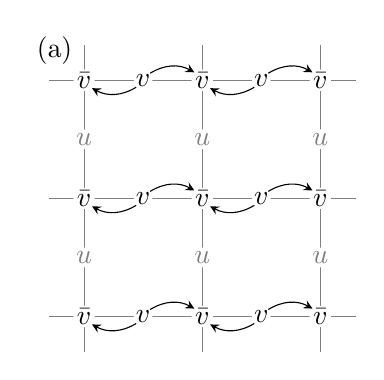
\begin{tikzpicture}[scale=1.5]
        \draw[help lines] (-0.3, -0.3) grid (2.3, 2.3);

        \foreach \x in {0,...,2}
            \foreach \y in {0,...,1}
            {
                \node[circle, inner sep=0pt, color=black!50, fill=white] at (\x, \y+0.5) {$u$};
            }
        \foreach \y in {0,...,2}
        {
            \foreach \x in {0,...,2}
                \node[circle, inner sep=0pt, fill=white] (av\x\y) at (\x, \y) {$\bar{v}$};
            \foreach \x in {0,...,1}
                \node[circle, inner sep=0pt, fill=white] (v\x\y) at (\x+0.5, \y) {$v$};
        }
        \path[-stealth] (v00.south west) edge[bend left] node[midway, below, yshift=+1pt] {} (av00.south east);
        \path[-stealth] (v10.south west) edge[bend left] node[midway, below, yshift=+1pt] {} (av10.south east);
        %\path[-stealth] (v20.south west) edge[bend left] node[midway, below, yshift=+1pt] {} (av20.south east);
        \path[-stealth] (v01.south west) edge[bend left] node[midway, below, yshift=+1pt] {} (av01.south east);
        \path[-stealth] (v11.south west) edge[bend left] node[midway, below, yshift=+1pt] {} (av11.south east);
        %\path[-stealth] (v21.south west) edge[bend left] node[midway, below, yshift=+1pt] {} (av21.south east);
        \path[-stealth] (v02.south west) edge[bend left] node[midway, below, yshift=+1pt] {} (av02.south east);
        \path[-stealth] (v12.south west) edge[bend left] node[midway, below, yshift=+1pt] {} (av12.south east);
        %\path[-stealth] (v22.south west) edge[bend left] node[midway, below, yshift=+1pt] {} (av22.south east);
        %\path[-stealth] (v03.south west) edge[bend left] node[midway, below, yshift=+1pt] {} (av03.south east);
        %\path[-stealth] (v13.south west) edge[bend left] node[midway, below, yshift=+1pt] {} (av13.south east);
        %\path[-stealth] (v23.south west) edge[bend left] node[midway, below, yshift=+1pt] {} (av23.south east);

        \path[-stealth] (v00.north east) edge[bend left] node[midway, below, yshift=+1pt] {} (av10.north west);
        \path[-stealth] (v10.north east) edge[bend left] node[midway, below, yshift=+1pt] {} (av20.north west);
        %\path[-stealth] (v20.north east) edge[bend left] node[midway, below, yshift=+1pt] {} (av30.north west);
        \path[-stealth] (v01.north east) edge[bend left] node[midway, below, yshift=+1pt] {} (av11.north west);
        \path[-stealth] (v11.north east) edge[bend left] node[midway, below, yshift=+1pt] {} (av21.north west);
        %\path[-stealth] (v21.north east) edge[bend left] node[midway, below, yshift=+1pt] {} (av31.north west);
        \path[-stealth] (v02.north east) edge[bend left] node[midway, below, yshift=+1pt] {} (av12.north west);
        \path[-stealth] (v12.north east) edge[bend left] node[midway, below, yshift=+1pt] {} (av22.north west);
        %\path[-stealth] (v22.north east) edge[bend left] node[midway, below, yshift=+1pt] {} (av32.north west);
        %\path[-stealth] (v03.north east) edge[bend left] node[midway, below, yshift=+1pt] {} (av13.north west);
        %\path[-stealth] (v13.north east) edge[bend left] node[midway, below, yshift=+1pt] {} (av23.north west);
        %\path[-stealth] (v23.north east) edge[bend left] node[midway, below, yshift=+1pt] {} (av33.north west);

        \node[black] at (-0.25, 2.25) {(a)};
    \end{tikzpicture}
    \label{fig:adv-x-ave}
    \end{subfigure}%
    \begin{subfigure}{0.33\textwidth}
        \centering
    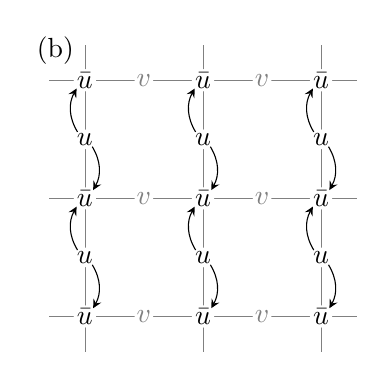
\begin{tikzpicture}[scale=1.5]
        \draw[help lines] (-0.3, -0.3) grid (2.3, 2.3);

        \foreach \x in {0,...,2}
        {
            \foreach \y in {0,...,1}
            {
                \node[circle, inner sep=0pt, fill=white] (u\x\y) at (\x, \y+0.5) {$u$};
            }
            \foreach \y in {0,...,2}
            {
                \node[circle, inner sep=0pt, fill=white] (au\x\y) at (\x, \y) {$\bar{u}$};
            }
        }
        \foreach \x in {0,...,1}
            \foreach \y in {0,...,2}
            {
                \node[circle, inner sep=0pt, color=black!50, fill=white] at (\x+0.5, \y) {$v$};
            }

        \path[-stealth] (u00.south east) edge[bend left] node[midway, below, yshift=+1pt] {} (au00.north east);
        \path[-stealth] (u10.south east) edge[bend left] node[midway, below, yshift=+1pt] {} (au10.north east);
        \path[-stealth] (u20.south east) edge[bend left] node[midway, below, yshift=+1pt] {} (au20.north east);
        %\path[-stealth] (u30.south east) edge[bend left] node[midway, below, yshift=+1pt] {} (au30.north east);
        \path[-stealth] (u01.south east) edge[bend left] node[midway, below, yshift=+1pt] {} (au01.north east);
        \path[-stealth] (u11.south east) edge[bend left] node[midway, below, yshift=+1pt] {} (au11.north east);
        \path[-stealth] (u21.south east) edge[bend left] node[midway, below, yshift=+1pt] {} (au21.north east);
        %\path[-stealth] (u31.south east) edge[bend left] node[midway, below, yshift=+1pt] {} (au31.north east);
        %\path[-stealth] (u02.south east) edge[bend left] node[midway, below, yshift=+1pt] {} (au02.north east);
        %\path[-stealth] (u12.south east) edge[bend left] node[midway, below, yshift=+1pt] {} (au12.north east);
        %\path[-stealth] (u22.south east) edge[bend left] node[midway, below, yshift=+1pt] {} (au22.north east);
        %\path[-stealth] (u32.south east) edge[bend left] node[midway, below, yshift=+1pt] {} (au32.north east);

        \path[-stealth] (u00.north west) edge[bend left] node[midway, below, yshift=+1pt] {} (au01.south west);
        \path[-stealth] (u10.north west) edge[bend left] node[midway, below, yshift=+1pt] {} (au11.south west);
        \path[-stealth] (u20.north west) edge[bend left] node[midway, below, yshift=+1pt] {} (au21.south west);
        %\path[-stealth] (u30.north west) edge[bend left] node[midway, below, yshift=+1pt] {} (au31.south west);
        \path[-stealth] (u01.north west) edge[bend left] node[midway, below, yshift=+1pt] {} (au02.south west);
        \path[-stealth] (u11.north west) edge[bend left] node[midway, below, yshift=+1pt] {} (au12.south west);
        \path[-stealth] (u21.north west) edge[bend left] node[midway, below, yshift=+1pt] {} (au22.south west);
        %\path[-stealth] (u31.north west) edge[bend left] node[midway, below, yshift=+1pt] {} (au32.south west);
        %\path[-stealth] (u02.north west) edge[bend left] node[midway, below, yshift=+1pt] {} (au03.south west);
        %\path[-stealth] (u12.north west) edge[bend left] node[midway, below, yshift=+1pt] {} (au13.south west);
        %\path[-stealth] (u22.north west) edge[bend left] node[midway, below, yshift=+1pt] {} (au23.south west);
        %\path[-stealth] (u32.north west) edge[bend left] node[midway, below, yshift=+1pt] {} (au33.south west);
        \node[black] at (-0.25, 2.25) {(b)};
    \end{tikzpicture}
    \label{fig:adv-y-ave}
    \end{subfigure}%
    \begin{subfigure}{0.33\textwidth}
        \centering
    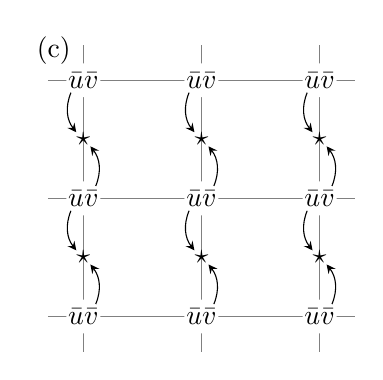
\begin{tikzpicture}[scale=1.5]
        \draw[help lines] (-0.3, -0.3) grid (2.3, 2.3);

        \foreach \x in {0,...,2}
            \foreach \y in {0,...,2}
                \node[circle, inner sep=0pt, fill=white] (uv\x\y) at (\x, \y) {$\bar{u}\bar{v}$};
        \foreach \x in {0,...,2}
            \foreach \y in {0,...,1}
                \node[circle, inner sep=0pt] (duv\x\y) at (\x, \y+0.5) {$\star$};

        \path[stealth-] (duv00.south east) edge[bend left] (uv00.north east);
        \path[stealth-] (duv10.south east) edge[bend left] (uv10.north east);
        \path[stealth-] (duv20.south east) edge[bend left] (uv20.north east);
        %\path[stealth-] (duv30.south east) edge[bend left] (uv30.north east);
        \path[stealth-] (duv01.south east) edge[bend left] (uv01.north east);
        \path[stealth-] (duv11.south east) edge[bend left] (uv11.north east);
        \path[stealth-] (duv21.south east) edge[bend left] (uv21.north east);
        %\path[stealth-] (duv31.south east) edge[bend left] (uv31.north east);
        %\path[stealth-] (duv02.south east) edge[bend left] (uv02.north east);
        %\path[stealth-] (duv12.south east) edge[bend left] (uv12.north east);
        %\path[stealth-] (duv22.south east) edge[bend left] (uv22.north east);
        %\path[stealth-] (duv32.south east) edge[bend left] (uv32.north east);
                                                                           
        \path[stealth-] (duv00.north west) edge[bend left] (uv01.south west);
        \path[stealth-] (duv10.north west) edge[bend left] (uv11.south west);
        \path[stealth-] (duv20.north west) edge[bend left] (uv21.south west);
        %\path[stealth-] (duv30.north west) edge[bend left] (uv31.south west);
        \path[stealth-] (duv01.north west) edge[bend left] (uv02.south west);
        \path[stealth-] (duv11.north west) edge[bend left] (uv12.south west);
        \path[stealth-] (duv21.north west) edge[bend left] (uv22.south west);
        %\path[stealth-] (duv31.north west) edge[bend left] (uv32.south west);
        %\path[stealth-] (duv02.north west) edge[bend left] (uv03.south west);
        %\path[stealth-] (duv12.north west) edge[bend left] (uv13.south west);
        %\path[stealth-] (duv22.north west) edge[bend left] (uv23.south west);
        %\path[stealth-] (duv32.north west) edge[bend left] (uv33.south west);
        \node[black] at (-0.25, 2.25) {(c)};
    \end{tikzpicture}
    \label{fig:adv-y-diff}
    \end{subfigure}%
    \caption{%
        A cross-section illustrating the steps in computing the $D_2[(A_2 u) (A_1 v)]$
        term of the first component of the advection. The horizontal and vertical
        velocity component discretization locations are marked by $u$ and $v$,
        respectively. Arrows emanate from a point contributing to a stencil and point to
        the center of the stencil.
        (a) $A_1$ averages $v$ in the $x$ direction, yielding an approximation $\bar{v}$
        at grid vertices (in 3D, centers of cell edges for which $x$ and $y$ are
        constant).
        (b) $A_2$ averages $u$ in the $y$ direction, yielding an approximation $\bar{u}$
        at the same points as (a). The quantities $A_1 v$ and $A_2 u$ are collocated and
        can be directly multiplied to obtain an approximation of $uv$ at locations marked
        $\bar{u}\bar{v}$.
        (c) $D_2$ approximately differentiates $uv$ in the $y$ direction, yielding the
        desired quantity at each point marked $\star$.
        The approximation of $uv$ is also used to compute $D_1[(A_1 v)(A_2 u)]$ in the
        second component of the advection, wherein application of $D_1$ instead yields
        approximations collocated with locations marked $v$ in (a).
    }
    \label{fig:discretization}
\end{figure}


To discretize the Navier-Stokes equations~\eqref{eq:ins-momentum}--\eqref{eq:ins-incomp},
we use a marker-and-cell (MAC) grid~\cite{Welch:1965jv}: for grid cell center $\x_i$,
scalar-valued function $s(\x)$ is discretized at $\x_i$, and component $\e_a\cdot\vec{v}$
of vector-valued function $\vec{v}(\x)$ at $\x_i - \sfrac12h\e_a$, where $\e_a$ is a
canonical basis vector. Define the centered difference operator
\begin{equation*}
    D_a\phi(\x) = \frac{\phi(\x+\sfrac12 h\e_a) - \phi(\x-\sfrac12 h\e_a)}{h},
\end{equation*}
for which, e.g., $D_1$ approximates differentiation in the $x$ direction. The discrete
divergence, gradient, and Laplacian operators use centered differences, resulting in a
2-point stencil for each discrete first derivative and the standard 7-point discrete
Laplacian. We also define the centered average operator
\begin{equation*}
    A_a\phi(\x) = \frac{\phi(\x+\sfrac12 h\e_a) + \phi(\x-\sfrac12 h\e_a)}2.
\end{equation*}
By averaging $u$ in the $y$ direction and $v$ in the $x$ direction, we obtain collocated
approximations to $u$ and $v$ at the center of a cell edge. Averaging, e.g., $u$ in the
$x$ direction yields an approximation to $u$ at the cell center. We can therefore
discretize the components of the advection term $\div(\u\otimes\u)$ by
\begin{equation}\label{eq:advection}
    \div[h](\u\otimes\u) := %D_b[H^{bl}_rH^{am}_s (A_l u^s(\x,\,t)) (A_m u^r(\x,\,t))].
    \left[\begin{array}{c}
        D_1[(A_1 u) (A_1 u)] + D_2[(A_1 v) (A_2 u)] + D_3[(A_1 w) (A_3 u)] \\
        D_1[(A_2 u) (A_1 v)] + D_2[(A_2 v) (A_2 v)] + D_3[(A_2 w) (A_3 v)] \\
        D_1[(A_3 u) (A_1 w)] + D_2[(A_3 v) (A_2 w)] + D_3[(A_3 w) (A_3 w)]
    \end{array}\right].
\end{equation}
The symbol $\div[h]$ represents the discrete divergence operator.  Figure~%
\ref{fig:discretization} illustrates the steps in computing $D_2[(A_1 v)(A_2 u)]$, which
appears in the first component in~\eqref{eq:advection}. Morinishi \latin{et al}.\ show
that this scheme, $Div. - S2$ in their parlance, is conservative under the assumption
that $\u$ is discretely divergence-free~\cite{Morinishi:1998us}.

To advance the solution, we use either the backward-forward Euler-based scheme~%
\cite{Ascher:1997tm} or the 2-stage scheme described by Peskin~\cite{Peskin:2002go},
modified to advance structures using the newest velocities. The modification makes these
schemes first-order in time, but allow us to separate the Eulerian update from the
Lagrangian update by requiring only information at the beginning of the timestep to
evaluate forces and moving the structure at the end of the timestep. For the
backward-forward Euler scheme, discretizing~\eqref{eq:ins-momentum} to advance time to
$t+\timestep$, yields linear solves of Helmholtz type,
\begin{equation}\label{eq:disc-momentum}
    (I - \timestep\rho^{-1}\mu \laplacian_h) \u^\ast = \u^n - \timestep\left[\div[h]\left(\u^n\otimes\u^n\right) + \rho^{-1}\left(\f^{n+1} - \grad[h]p^n\right)\right] \quad\text{in}~\domain, \\
\end{equation}
with boundary conditions
\begin{equation}\label{eq:disc-bdy}
    \u^\ast = \u^{n+1}_b + \timestep \grad[h] q^{n} \quad\text{on}~\partial\domain,
\end{equation}
where superscripts denote the time step, $\u_b$ is velocity boundary data, $\laplacian_h$
and $\grad[h]$ are the discrete Laplacian and gradient, respectively, and $q$ is
described below. The force density $\f^{n+1}$ is advanced explicitly. The intermediate
velocity field $\u^\ast$ may not be divergence-free. To obtain a velocity field that
satisfies~\eqref{eq:ins-incomp}, we use projection method II (PmII) of Brown, Cortez, and
Minion~\cite{Brown:2001bq}. PmII updates the pressure
\begin{equation*}
    p^{n+1} = p^n + (\rho I - \timestep\mu\laplacian_h)q^{n+1},
\end{equation*}
and generates the divergence-free velocity field
\begin{equation}\label{eq:vel-update}
    \u^{n+1} = \u^\ast - \timestep\grad[h]q^{n+1}
\end{equation}
using pseudo-pressure $q^{n+1}$, which satisfies
\begin{equation}
\begin{alignedat}{2}
    &\alpha k \laplacian_h q^{n+1} = \div[h]\u^\ast &&\quad \text{in}~\domain, \\
    &\n\cdot\grad[h] q^{n+1} = 0                    &&\quad \text{on}~\partial\domain.
\end{alignedat}
\end{equation}
The velocity update~\eqref{eq:vel-update} provides the boundary conditions~%
\eqref{eq:disc-bdy} using a lagged value of the pseudo-pressure. The 2-stage RK method
consists of a backward-forward Euler step followed by a Crank-Nicolson-midpoint step,
which involves only minor modifications to~\eqref{eq:disc-momentum}. In total, we perform
3 Helmholtz solves and 1 Poisson solve per RK stage.

We employ preconditioned conjugate gradients (PCG) to perform the solves. We use
Chebyshev iteration as a preconditioner for the Helmholtz solves and as an error
smoothing procedure and direct solver for multigrid (MG) to precondition the Poisson
solve. Chebyshev iteration is a generalization of weighted Jacobi iteration which
requires only the ability to perform sparse matrix polynomial-vector multiplication.
Chebyshev iteration (MG) PCG is therefore parallelized by using a parallel sparse
matrix-vector multiplication routine with Horner's method to evaluate the polynomials.

In the case of a triply periodic domain, it is clear that the linear solves involve
symmetric matrices. For Dirichlet or Neumann boundaries, we extrapolate using values at
the neighboring grid points and boundary data to fill ghost points. In these situations,
the standard discrete second derivative may actually approximate some non-unit multiple
of its continuous counterpart near the boundary. To account for this but maintain
symmetry of the Helmholtz matrices, we scale equations involving near-boundary values,
excluding the offending discrete second derivative and ghost cell terms. The trade-off is
3 extra diagonal matrix-vector multiplications per RK stage for the ability to use PCG
for the linear solves. For details, see~\ref{sec:boundary-correction}.

% vim: cc=90 tw=89

\section{Cell energy and power models}\label{sec:energy}

In this section, we describe the various forms of energy density (energy per area) and power density (power per
area) used in our simulations, and give analytic expressions for each. The corresponding force densities are given
in~\ref{sec:forces}. We use five kinds of densities: spring energy, damped spring power, tension energy,
dissipative power, and Canham-Helfrich bending energy. For constitutive law $W$, we define the functional
\begin{equation}
    \energy[\X, \U] = \int\limits_\interface W(\X, \U, \ldots) \d\X,
\end{equation}
where the ellipsis indicates that $W$ may depend on spatial derivatives of $\X$ or $\U$. The force density
associated with $W$ is found by computing the first variation of $\energy$,
\begin{equation}
    \F = -\delta\energy,
\end{equation}
with respect to $\X$ for energy densities and to $\U$ for power densities. Because our ultimate goal is a
three-dimensional simulation, we limit our descriptions to the three-dimensional case. Considerations for the
two-dimensional case are treated elsewhere~\cite{Peskin:2002go,Erickson:2010uzba}.

We begin with Hookean energy and damped spring power density. These have the simplest constitutive laws we use,
depend only on surface locations and surface velocities, and take the form
\begin{equation}
        W_\text{Hk}(\X) = \frac{k}2 {\|\X - \X'\|}^2\quad\text{and}\quad
        W_\text{damped}(\U) = \frac{\eta}2{\|\U - \U'\|}^2,
\end{equation}
where $\X'=\X'(\theta, \varphi, t)$ is the tether location for $\X(\theta, \varphi, t)$,
$\U'=\U'(\theta, \varphi, t)$ is the prescribed velocity of the tether point, $k$ is the spring constant, and
$\eta$ is the damping constant.  Due to the lack of information about the mechanical properties of endothelial
cells, we model the endothelium as a rigid, stationary object with $\ethm{k}=2.5\dynpercm$ and
$\ethm\eta=2.5\sci{-7}\dynsecpercm$, chosen to be as large as possible for the chosen spatial and temporal step
size with prescribed velocity $\U' = \vec{0}$. We compare different choices for $\X'$ in \cref{sec:whole-blood}.

Next, we consider the tension energy densities for RBCs and platelets. These penalize stretching and areal
dilation of the cell membranes. Let $\lambda_1$ and $\lambda_2$ be the principal extensions, \latin{i.e.}, the
maximal and minimal ratios of stretching relative to a reference configuration. We define the invariants
$I_1=\lambda_1^2+\lambda_2^2-2$ and $I_2 = \lambda_1^2\lambda_2^2-1$, which measure relative changes in length and
area, respectively, such that $I_1 = I_2 = 0$ correspond to a rigid body motion. We express the tension density in
terms of these invariants. Skalak's Law was designed specifically for RBCs~\cite{Skalak:1973tp}:
\begin{equation}\label{eq:skalak-law}
    W_\text{Sk}(I_1, I_2) = \frac{E}4\left(I_1^2 + 2I_1 - 2I_2\right) + \frac{G}4 I_2^2.
\end{equation}
$E$ is the shear modulus, and $G$ is the bulk modulus. For RBCs, we follow Fai \latin {et al.}~\cite{Fai:2013do} and set $\rbc{E} = 2.5\sci{-3}\dynpercm$ and $\rbc{G} = 2.5\sci{-1}\dynpercm$. We use
the shape given by Evans \& Fung~\cite{Evans:1972uf} for the reference RBC with radius $R_0 = 3.91\um$,
\begin{equation}
    \rbc{\vec{\hat{X}}}(\theta, \varphi) = R_0\begin{bmatrix}
            \cos\theta\cos\varphi \\
            \sin\theta\cos\varphi \\
            z(\cos\varphi)\sin\varphi
    \end{bmatrix},
\end{equation}
where $(\theta, \varphi)\in(-\pi, \pi]\times[-\pi/2, \pi/2]$ and $z(r) = 0.105 + r^2 - 0.56r^4$. Platelets, on the
other hand, do not have a purpose-built constitutive law, but are known to be stiffer than RBCs. We use the neo-Hookean model
\begin{equation}\label{eq:neohookean}
    W_\text{nH}(I_1, I_2) = \frac{E}2\left(\frac{I_1+2}{\sqrt{I_2+1}}-2\right) + \frac{G}2 {\left(\sqrt{I_2+1}-1\right)}^2
\end{equation}
with $\plt{E} = 1\sci{-1}\dynpercm$ and $\plt{G} = 1\dynpercm$, and an ellipsoidal reference configuration~%
\cite{Frojmovic:1982wk}
\begin{equation}
    \plt{\hat{\vec{X}}}(\theta, \varphi) = \begin{bmatrix}
            1.55\um\cos\theta\cos\varphi \\
            1.55\um\sin\theta\cos\varphi \\
            0.5\um\sin\varphi
    \end{bmatrix}.
\end{equation}

Platelets and RBCs also respond to changes in membrane curvature. Let $H$ be the membrane's mean curvature. The
Canham-Helfrich bending energy density takes the form~\cite{Canham:1970wx}
\begin{equation}\label{eq:bending-energy}
    W_\text{CH}(H) = 2\kappa {(H-H')}^2,
\end{equation}
where $\kappa$ is the bending modulus in units of energy, and $H'$ is the spontaneous or \emph{preferred}
curvature. An RBC generates a relatively weak response to changes in its curvature. Its bending modulus is
estimated to be in the range $0.3$--$4\sci{-12}\erg$~\cite{Mohandas:1994tg}. We use a bending modulus of
$\rbc\kappa = 2\sci{-12}\erg$ and a preferred curvature $H' = 0$ for RBCs. RBCs, therefore, tend to locally
flatten their membranes. For platelets, we use a larger bending modulus of $\plt\kappa=2\sci{-11}\erg$
and a preference for its reference curvature. Together with the neo-Hookean tension above, this maintains a fairly
rigid platelet.

Finally, we consider dissipative power, which causes the membrane to exhibit a viscoelastic response to strain. It
takes the form~\cite{Rangamani:2012hi}
\begin{equation}\label{eq:dissip-energy}
    W_\text{dissip}(\dot{\lambda}_1, \dot{\lambda}_2) = \frac{\nu}{2}\left(\frac{\dot{\lambda}_1^2}{\lambda_1^2} + \frac{\dot{\lambda}_2^2}{\lambda_2^2}\right),
\end{equation}
where $\nu$ is the membrane viscosity, and $\dot{\lambda}_i$ is the rate of change of $\lambda_i$. We imbue only
the RBC with viscoelasticity. We find this effective in eliminating some numerical instabilities. While Evans \&
Hochmuth suggest a viscosity of approximately $1\sci{-3}\dynsecpercm$~\cite{Evans:1976tx}, we find this to be
prohibitively expensive in practice, due to time step restrictions, and instead use
$\rbc\nu = 2.5\sci{-7}\dynsecpercm$.


\section{Geometry of reconstructed surfaces}\label{sec:rbfs}

From the previous section, we have analytic expressions for the energy density, and consequently the Lagrangian force density,
$\F$ (see Appendix B). The RBC and platelet force models require first and second derivatives along their
surfaces. Additionally, the IB force spreading operation requires quadrature weights for
the surfaces. This section finishes where we left off by discussing the construction of
the necessary discrete linear operators and quadrature weights $\weight[j]$ through the
use of RBF-based methods.

\subsection{Surface reconstruction with radial basis functions}\label{sec:rbf-interpolation}

Radial basis functions (RBFs) are a meshfree approach to scattered data approximation
where structural information is encoded purely as point-wise distances. With some
exceptions, they are an appropriate tool for interpolation at arbitrary locations. This
contrasts with, \latin{e.g.}, polynomials, where points must be chosen at grid vertices,
or spherical harmonics, for which special node sets are typically used. RBFs are a viable
approach for representing cells on par with Fourier methods~\cite{Shankar:2013ki}. They
are therefore appealing for representing blood cells.

Because our choice of force model for the endothelium does not require geometric
information, we limit the discussion to RBCs and platelets, which are topologically
spherical. The 2-sphere, $\sphere$, has parametrization
\begin{equation*}
    \Xp(\theta,\,\varphi) =
    \left[\begin{array}{c}
        \cos\theta\cos\varphi \\
        \sin\theta\cos\varphi \\
        \sin\varphi
    \end{array}\right],
\end{equation*}
$(\theta,\,\varphi)\in(-\pi,\,\pi]\times[-\pi/2,\,\pi/2]$.
Let $\data\sites = \{(\data\theta_i,\,\data\varphi_i)\}$ be a set of $\data\cardinality$
distinct \emph{data sites}, defined by the Bauer spiral~\cite{Bauer:2000km},
\begin{equation}\label{eq:bauer-spiral}
    \begin{aligned}
        &\varphi_j = \sin^{-1}(-1 + (2i + 1) / N), \\
        &\theta_j = \modulo\left(\sqrt{N\pi}\varphi_j + \pi,\,2\pi\right) - \pi,
    \end{aligned}
\end{equation}
where $N$ is the number of points, and $\modulo(a,\,b) = a - b\floor{a/b}$ is the modulo
function. Let $\data\Xp_i = \Xp(\theta_i,\,\varphi_i)$ for each
$(\theta_i,\,\varphi_i) \in \data\sites$. Suppose we wish to approximate $\psi(\Xp)$,
defined on $\sphere$. From \emph{basic function} $\phi$, we form our interpolatory basis
with the RBFs $\phi(\|\Xp-\data\Xp_i\|)$, $i=1,\,\ldots,\,\data\cardinality$. Attractive
choices for $\phi$ are the polyharmonic splines (PHS),
\begin{equation*}
    \text{PHS:}\quad\phi(r) = \begin{cases}
        r^{2k} \log r, \\
        r^{2k+1},
    \end{cases}
    \quad\text{for}\ k\in\mathbb{N},
\end{equation*}
which do not require a shape parameter, unlike Gaussian or multiquadric kernels~%
\cite{Fasshauer:2007ui}. However, PHS are finitely differentiable and conditionally
positive definite; they require additional polynomial terms up to degree $k$ to guarantee
a unique interpolant. Heuristically, $\data\cardinality$ is chosen so that data sites
outnumber polynomials at least 2-to-1 to maintain reasonable conditioning. On $\sphere$,
the polynomials are spherical harmonics. We denote the polynomials by $p_k(\Xp)$,
$k=1,\,\ldots,\,\poly\cardinality$. The interpolant takes the form
\begin{equation}\label{eq:rbf-interp}
    s(\Xp)
    = \sum_{i=1}^{\data\cardinality} c_i \phi(\|\Xp-\data\Xp_i\|)
    + \sum_{k=1}^{\poly\cardinality} d_k p_k(\Xp),
\end{equation}
and exactly recovers $\psi$ at each of the data sites,
$s(\data\Xp_j) = \psi(\data\Xp_i)$, for $j = 1,\,\ldots,\,\data\cardinality$. We further
constrain the coefficients $c_i$ so that the polynomials recover polynomial data,
\begin{equation}
    \sum_{i=1}^{\data\cardinality} c_i p_k(\data\Xp_i) = 0.
    \label{eq:constraints}
\end{equation}
Collecting the values $\Phi=(\phi(\|\data\Xp_j-\data\Xp_i\|))$, $P=(p_k(\data\Xp_j))$,
$\arr{c} = (c_i)$, $\arr{d} = (d_k)$, and $\arr{\psi} = (\psi(\data\Xp_j))$, we form
the dense symmetric block system
\begin{equation}\label{eq:rbf-interp-matrix}
    \left[\begin{array}{cc}
            \Phi & P \\ P^T & 0
    \end{array}\right]\left[\begin{array}{c}
            \arr{c} \\ \arr{d}
    \end{array}\right] = \left[\begin{array}{c}
            \arr{\psi} \\ \arr{0}
    \end{array}\right],
\end{equation}
where the matrix block $0$ is the $\poly\cardinality\times\poly\cardinality$ zero matrix
and $\arr{0}$ is a vector of $\poly\cardinality$ zeros. Because $\data\sites$ is fixed,
we need only construct this matrix and compute its factors once.

For RBC and platelet parametrizations, we identify the point $\X(\theta,\,\varphi,\,t)$
on $\interface$ with the point $\Xp(\theta,\,\varphi)$ on $\sphere$. Each component of
$\X$ is a function defined on $\sphere$. By sampling $\X$ at each point in $\data\sites$,
we can approximately reconstruct the surface by interpolating each of the components. It
is clear from Equations~\eqref{eq:skalak-law}--\eqref{eq:dissip-energy} that computing
the force densities requires values of $I_1$, $I_2$, and $H$, among others. These values
are derived from the first and second derivatives of $\X$. See~\ref{sec:forces} for
details. To meet the smoothness requirements for evaluating the force densities, we use
$\phi(r) = r^7$ for RBCs and platelets, with up to $5\th$ order spherical harmonics for
RBCs and just the constant polynomial for platelets. While this does not guarantee a
unique interpolant for the platelet, the resulting system~\eqref{eq:rbf-interp-matrix} is
invertible nonetheless. The interpolants are then thrice differentiable. We next describe
the construction of the necessary discrete differential operators.

\subsection{Discrete linear surface operators}

Let $\L$ be a linear operator. In particular, we are interested in the first- and
second-order partial differential operators, $\partial/\partial\theta$,
$\partial^2/\partial\theta\partial\varphi$, \latin{etc}. We approximate $\L\psi$ by
applying $\L$ analytically to the interpolant $s$ defined in Equation~%
\eqref{eq:rbf-interp}. This is straightforward, given a parametrized metric. For
$\sphere$, this is
\begin{equation}\label{eq:sphere-metric}
    \begin{aligned}
    \|\Xp(\theta_j,\,\varphi_j) - \Xp(\theta_i,\,\varphi_i)\|
    &= \sqrt{2(1 - \cos\varphi_j\cos\varphi_i\cos(\theta_j-\theta_i) - \sin\varphi_j\sin\varphi_i)} \\
    &= \sqrt{2(1-\Xp(\theta_j,\,\varphi_j)\cdot\Xp(\theta_i,\,\varphi_i))}.
\end{aligned}
\end{equation}
However, evaluating $\L s$ at each data site involves dense operations against a
$\data\cardinality\times(\data\cardinality+\poly\cardinality)$ matrix. Depending on the
needs of the simulation, the number of data sites may be large.  In the interest of
saving memory and time for such cases, we opt instead to use fewer data sites to
reconstruct the surface, and choose a larger set of $\sample\cardinality$ \emph{sample
sites}, $\sample\sites$, at which to evaluate $\L$. We must then also consider $\L$ the
identity operator in order to obtain $\X$ at sample sites. Evaluating $\L s$ at each
sample site and collecting values $\L\Phi = (\L\phi(\|\Xp-\data\Xp_i\|)|_{\Xp=\Xpsj})$
and $\L P = (\L p_k(\Xp)|_{\Xp=\Xpsj})$, where $\Xpsj = \Xp(\theta_j,\,\varphi_j)$ for
each $(\theta_j,\,\varphi_j)\in\sample\sites$,\comment{}{$\Xpsj$ is \emph{not} a sample
site, but $(\theta_j,\,\varphi_j)\in\sample\sites$ is.} we have
\begin{equation}\label{eq:rbf-operator}
    \begin{aligned}
    \left[\begin{array}{cc}
            \L\Phi & \L P
    \end{array}\right]\left[\begin{array}{c}
            \arr{c} \\ \arr{d}
    \end{array}\right] &\hphantom{:}=
    \left[\begin{array}{cc}
            \L\Phi & \L P
    \end{array}\right]\left[\begin{array}{cc}
            \Phi & P \\ P^T & 0
    \end{array}\right]^{-1}\left[\begin{array}{c}
            \arr{\psi} \\ \arr{0}
    \end{array}\right] \\ &:=
    \left[\begin{array}{cc}
            L & \ast
    \end{array}\right]\left[\begin{array}{c}
            \arr{\psi} \\ \arr{0}
    \end{array}\right],
\end{aligned}
\end{equation}
where we have used Equation~\eqref{eq:rbf-interp-matrix} to substitute for $\arr{c}$ and
$\arr{d}$. The matrix $L$ is the discrete analogue of $\L$ applied at each sample site.
It is important to note that $L$ is completely independent of the function $\psi$; in
fact, it depends only on the functions $\phi$ and $p_k$, the fixed data sites
$\data\sites$, and the fixed sample sites $\sample\sites$.  The block marked by $\ast$ is
multiplied by zeros, and can be discarded. We compute a separate $L$ for each operator
$\L$ as a preprocessing step, and simply apply these matrices to any function that needs
to be evaluated or differentiated. It is also straightforward to generate versions of $L$
that produce derivatives at the data sites simply by replacing $\Xpsj$ with $\data\Xp_j$
in the above discussion. With these operators in hand, the force densities are readily
discretized. The quantities $I_1$, $I_2$, and $H$ in Section~\ref{sec:energy} are
calculated using local first and second derivatives. Application of the dense discrete
differential operators is performed in parallel with a parallel implementation of
\texttt{BLAS}. Lagrangian forces can therefore be computed in parallel with few thread
synchronizations.

We now have a method for computing a suitable set of points and for discretizing $\F$ for
use in~\eqref{eq:ib-spread}. To compute a force from a force density, we need to
approximate quadrature weights, or surface patch areas, for each sample site. The
following section is devoted to computing quadrature weights $\weight[j]$ for each
sample site using RBFs.

% vim: cc=90 tw=89

\subsection{Surface area weights via RBF quadrature}\label{sec:rbf-quadrature}

We also use the known parametrization of $\sphere$ to compute RBF-based quadrature weights
on $\sphere$ as a preliminary step in computing quadrature weights on any surface
diffeomorphic to $\sphere$, namely, RBC and platelet membranes.

As before, consider a function $\psi(\Xp):\sphere \to \mathbb{R}$, and $\phi: \sphere \times \sphere \to \mathbb{R}$ be a radial kernel defined on the sphere. We wish to find a set
of quadrature weights $\omega_j$ such that
\begin{equation}\label{eq:quad-desire}
    \int_{\sphere} \psi(\Xp) \d\Xp \approx \sum_{j=1}^{\sample\cardinality} \omega_j \psi(\Xpsj).
\end{equation}
We use a variant of the technique described by Fuselier \latin{et al.}~%
\cite{Fuselier:2013coba}.  Choosing $\psi(\Xp) = \phi(\|\Xp-\sample\Xp_i\|)$ for each
$\sample\Xp_i$, Equation~\eqref{eq:quad-desire} becomes
\begin{equation}
    \sum_{j=1}^{\sample\cardinality} \omega_j \phi(\|\Xpsj-\sample\Xp_i\|)
    \approx \int_{\sphere}\phi(\|\Xp-\sample\Xp_i\|) \d\Xp := \L\phi|_{\Xp=\sample\Xp_i}.
    \label{eq:cond1t}
\end{equation}
However, because the spherical metric~\eqref{eq:sphere-metric} depends only on the angle
between two points, $\L\phi$ is constant over
the sphere. We therefore expect the right-hand side to be a constant, which we denote
$-I_\phi$. We require further that $\omega_j$ sum to the surface area of $\sphere$,
\latin{i.e.},
\begin{equation}
    \sum_{j=1}^{\sample\cardinality} \omega_j  = 4\pi.
    \label{eq:weight-sum}
\end{equation}
Treating $I_\phi$ as an unknown scalar, we rewrite the constraints~\eqref{eq:cond1t} and%
~\eqref{eq:weight-sum} as a symmetric block linear system for $\omega_j$. Let
$\Phi = (\phi(\|\Xpsj - \sample\Xp_i\|))$, $\arr{\omega} = (\omega_j)$, $\arr{0}$ 
be a vector of $\sample\cardinality$ zeros, and $\arr{1}$ be defined similarly with ones.
Then
\begin{equation}\label{eq:rbf-quadrature}
    \left[\begin{array}{cc}
            \Phi & \arr{1} \\ \arr{1}^T & 0
    \end{array}\right]\left[\begin{array}{cc}
            \arr{\omega} \\ I_\phi
    \end{array}\right] = \left[\begin{array}{c}
            \arr{0} \\ 4\pi
    \end{array}\right].
\end{equation}
$I_{\phi}$ serves as a Lagrange multiplier that enforces~\eqref{eq:weight-sum}, and
$-I_\phi$ is a good approximation to $\L\phi$. By choosing $\phi(r) = r$, we guarantee a
unique solution and obtain weights that we observe to converge at 3\textsuperscript{rd}
order. It is possible to improve the order of the quadrature weights by increasing the
order of the PHS RBF at the potential cost of poorer conditioning and either loss of
invertibility or requiring knowledge of higher-order moments~\cite{Fuselier:2013coba}.

Having described the computation of quadrature weights for $\sphere$, we now
describe how to compute quadrature weights for $\interface$, which has parametrization
$\X(\theta,\,\varphi)$ and Jacobian $J(\theta,\,\varphi)$. The point
$\X(\theta,\,\varphi)$ on the cell and $\Xp(\theta,\,\varphi)$ share surface coordinates
and the determinant of the Jacobian for the spherical coordinate mapping (for radius 1) is simply $\cos\varphi$.  We use a change of variables to
express the infinitesimal area $\d\X$ as
\begin{equation}\label{eq:quad-cov}
    \d\X
    = J(\theta,\,\varphi)\d\qs
    = J(\theta,\,\varphi)\sec\varphi\d\Xp,
\end{equation}
where $\d\qs$ is an infinitesimal area in parameter space. The weights $\omega_j$ found
above are discrete analogues of $\d\Xp$ at $\sample\Xp_j$. The discrete analogue of
$\d\qs$ at the $j^\text{th}$ sample site,
\begin{equation*}
    \sigma_j=\sec\varphi_j\omega_j,
\end{equation*}
can be computed at the outset of a simulation. To avoid numerical issues, we require that
$\cos\varphi_j \neq 0$ for each sample site. This is true everywhere on $\sphere$ except
the poles, $(0,\,0,\,\pm1)$. The Bauer spiral~\eqref{eq:bauer-spiral} conveniently avoids
these points. We now arrive our weights for $\interface$. At $\X_j$, we have
\begin{equation}
    \weight[j] = \sigma_j J_j,
\end{equation}
where $J_j = J(\theta_j,\,\varphi_j)$. Computing $\weight[j]$ given $\sigma_j$ and $J_j$
amounts to a single multiplication, which can be done trivially in parallel.

%The methods described in this section are not restricted to the sphere. In Section~%
%\ref{sec:whole-blood}, we simulate the endothelium, which is a topological torus, due to
%the periodicity of the domain. Though we do not need geometric information for the force
%model used for the endothelium, the RBF methods above are also applicable to the torus,
%and therefore the endothelium. The following section describes the necessary
%modifications for the endothelium. We use a local variation of these methods as part of
%the simulation initialization process, described in Section~\ref{sec:blood-init}.


%\subsection{A note on the endothelium}
%While our choice of force density for the endothelium does not require surface
%reconstruction or quadrature weights, the methods described above are equally applicable.
%The periodicity of $\domain$ makes the endothelium a topological torus. The 4-dimensional
%torus, $\mathbb{T}$, with parametrization
%\begin{equation*}
%    \Xp(\theta,\,\varphi) = \left[\begin{array}{c}
%            \cos\theta\\ \sin\theta \\ \cos\varphi \\ \sin\varphi
%    \end{array}\right],
%\end{equation*}
%for $\theta,\,\varphi\in[0,\,2\pi)$, is orientation agnostic and homogeneous. It has
%surface area $4\pi^2$ and Jacobian $\tilde{J} = 1$. It is, however, trivial to choose a
%set of points on $\mathbb{T}$ that generate equal quadrature weights without the need to
%solve a system like~\eqref{eq:rbf-quadrature}. Any regular grid suffices, but we generate
%a set of $N$ points, whether used for interpolation or not, with the spiral
%\begin{align*}
%    \varphi_i &= 2\pi (i-1)/N, \\
%    \theta_i &= \modulo\left(\left\lceil\!\sqrt{N}\mskip\thinmuskip\right\rceil\varphi_i,\,2\pi\right).
%\end{align*}
%Using distances between points
%on $\mathbb{T}$ to construct RBFs allow for the interpolation of, and quadrature on, any
%toroidal surface. However, care needs to be taken in applying the constructed discrete
%operators to a ``flat'' torus, such as the endothelium. If, for example, $L$ is the
%discrete analog of $\L$ evaluated at sample site $(\sample\theta,\,\sample\varphi)$ and
%the interpolated function $\psi(\theta,\,\varphi)$ decomposes into
%\begin{equation*}
%    \psi(\theta,\,\varphi) = \bar{\psi}(\theta,\,\varphi) + \text{periodic part},
%\end{equation*}
%where $\bar{\psi}$ is known, aperiodic, and independent of time, then
%\begin{equation*}
%    \L\psi(\sample\theta,\,\sample\varphi)
%    \approx \L\bar{\psi}(\sample\theta,\,\sample\varphi) + L\left(\data{\vec{\psi}} - \data{\vec{\bar{\psi}}}\right)
%    := L\data{\vec{\psi}} + \epsilon,
%\end{equation*}
%where $\data{\vec{\psi}}$ and $\data{\vec{\bar{\psi}}}$ are vectors formed by evaluating
%$\psi$ and $\bar{\psi}$, respectively, at each point in $\data\sites$. Computing
%$\epsilon$ for each sample site can be done simultaneously, resulting in the vector
%$\vec{\epsilon}$. A correction like $\vec{\epsilon}$ may be needed for each linear
%operator.


\section{Results}\label{sec:results}

We have taken a number of departures from the traditional application of the IB method and RBC models. In the
following sections, we establish convergence for our implementation of RBF-IB, demonstrate its energy dissipation properties, demonstrate impermeability of the
RBCs, and observe typical RBC behaviors before presenting the results of our whole blood simulations.

\subsection{Convergence study}\label{sec:convergence}

In this section, we perform a series of tests on a single perturbed RBC undergoing
relaxation. We simplify the RBC model and use only Skalak's Law. We expect the IB method
to approximate the fluid velocity at first order for thin shells, as it cannot recover
the pressure jump across the interface. We stretch the RBC by a factor of 1.1 in the $z$
direction and compress it in the $x$ direction to maintain its reference volume. We place
the cell in the center of a $16\um\times16\um\times16\um$ domain with homogeneous
Dirichlet boundary conditions in the $y$ direction and periodic boundaries elsewhere. The
fluid velocity is initially zero. The cell is then allowed to relax for $180\us$.

We use the 3-point kernel $\hat{\Dirac}_1$ derived by Roma \latin{et al.}~%
\cite{Roma:1999tx} for spreading and interpolation and the 2-stage RK method described in
Section~\ref{sec:ib} to advance the fluid velocity. Fluid grids are chosen to have $20r$
grid points per $16\um$ in each direction for $r$ from 1 to 6. On successive grids, we
compare the fluid velocity at cell centers in a regular grid of $20^3$ cells and surface
positions at 1000 surface points. For convergence of order $p$, we expect the ratio of
successive errors to satisfy
\begin{equation}
    \frac{\epsilon_r}{\epsilon_{r+1}} = \left|\frac{((r+1)/r)^p-1}{((r+2)/(r+1))^{-p}-1}\right|,
\end{equation}
which we solve numerically to determine $p$. We compute the errors in $\X$ using discrete
versions of the $L_2$ and $L_\infty$ norms,
\begin{gather}
    \|\X(\theta,\,\varphi)\|_2^2 =
    \int\limits_{\sphere} \X(\theta,\,\varphi)\cdot\X(\theta,\,\varphi) \d\qs \quad\text{and} \\
    \|\X(\theta,\,\varphi)\|_\infty^2 =
    \max_{(\theta,\,\varphi)} \X(\theta,\,\varphi)\cdot\X(\theta,\,\varphi),
\end{gather}
respectively.

Tables~\ref{tab:u-rbc-conv} and~\ref{tab:x-rbc-conv} show $L_2$ and $L_\infty$ errors in
$\u$ and $\X$ between successive grids. We observe first-order convergence, as expected.
Satisfied with the convergence of our implementation, we henceforth continue using the
Bauer spiral to discretize RBCs and use the complete RBC model, which we verify in the
next section.

\begin{table}[tbp]
    \centering
    \caption[Convergence of fluid velocities for relaxing RBC test]{%
Convergence of $\u$ for a sequence of grids. The refinement ratio $r$, defined as the
refinement in $h$ relative to the coarsest grid, determines the simulation parameters:
$rh = 0.8\um$ and $r\timestep = 180\ns$. Errors are computed between grids of refinement
factor $r$ and $r+1$. Values of $\u$ are sampled at $t = 180\us$ at cell centers on the
coarsest grid.
    }\label{tab:u-rbc-conv}
    \begingroup
    \setlength{\tabcolsep}{9pt}
    \renewcommand{\arraystretch}{1.5}
    \begin{tabular}{c|cc|cc}
                                                                                     \toprule
        $r$ & $L_2$ error            & order   & $L_\infty$ error       & order   \\ \midrule
        1   & $\scinot{1.74592}{-3}$ &         & $\scinot{1.59995}{-2}$ &         \\
        2   & $\scinot{9.92788}{-5}$ &         & $\scinot{6.52038}{-4}$ &         \\
        3   & $\scinot{3.65264}{-5}$ & 6.85983 & $\scinot{3.34322}{-4}$ & 1.06075 \\
        4   & $\scinot{2.31069}{-5}$ & 2.87612 & $\scinot{2.30732}{-4}$ & 1.60689 \\
        5   & $\scinot{1.65898}{-5}$ & 1.25668 & $\scinot{2.28193}{-4}$ & 0.83030 \\ \bottomrule
    \end{tabular}
    \endgroup
\end{table}

\begin{table}[tbp]
    \centering
    \caption[Convergence of surface positions for relaxing RBC test]{%
Convergence of $\X$ for a sequence of grids. The refinement ratio $r$, defined as the
refinement in $h$ relative to the coarsest grid, determines the simulation parameters:
$r\timestep = 180\ns$, $n_d = 125r^2$, and $n_s = 500r^2$. Errors are computed between
grids of refinement factor $r$ and $r+1$. Values of $\X$ are sampled at $t = 180\us$ at
$1000$ Bauer spiral points.
    }\label{tab:x-rbc-conv}
    \begingroup
    \setlength{\tabcolsep}{9pt}
    \renewcommand{\arraystretch}{1.5}
    \begin{tabular}{c|cc|cc}
                                                                                     \toprule
        $r$ & $L_2$ error            & order   & $L_\infty$ error       & order   \\ \midrule
        1   & $\scinot{6.05447}{-3}$ &         & $\scinot{2.68249}{-3}$ &         \\
        2   & $\scinot{1.61678}{-3}$ &         & $\scinot{6.86140}{-4}$ &         \\
        3   & $\scinot{7.69150}{-4}$ & 2.74664 & $\scinot{3.30734}{-4}$ & 2.86457 \\
        4   & $\scinot{4.66203}{-4}$ & 1.89474 & $\scinot{1.86139}{-4}$ & 1.84435 \\
        5   & $\scinot{2.82578}{-4}$ & 1.46574 & $\scinot{1.18713}{-4}$ & 1.82742 \\ \bottomrule
    \end{tabular}
    \endgroup
\end{table}

\subsection{Energy Estimates}\label{sec:energy-est}

As mentioned in Section~\ref{sec:rbfib}, the RBF-IB method uses different sets of
Lagrangian points for spreading forces and updating immersed structures. We now track the
total energy of the combined fluid-RBC system in the relaxation test just described.
This energy is given as 
\begin{align}
    E = \int_\domain \left[\frac{\density}2\u\cdot\u + \int_\interface \Dirac(\x-\X)W_\text{Sk}(\X,\,\ldots)\d\X\right] \d\x.
\label{eq:energy}
\end{align}
The first term corresponds to the energy of the fluid, and the second to the energy of
the structure. Since the relaxation test involves an initial increase in kinetic energy
of the fluid followed by a gradual dissipation of the potential energy of the RBC as it
relaxes according to the Skalak law, we expect the total energy of the system to decrease
over time. We plot a discretized version of the energy~\eqref{eq:energy} as a function of
time in Figure~\ref{fig:energies} for refinement factors $r=5$ and $r=6$. Figure~%
\ref{fig:energies} clearly shows that our method dissipates energy in the manner expected
in this problem.  We also observed that the RBF-IB method was stable for representing
RBCs and platelets in whole blood simulations.

\begin{figure}[tbp]
\centering
\begin{tikzpicture}
\begin{groupplot}[
    group style={
        y descriptions at=edge left,
        group name=energy,
        group size=2 by 1
    },
    width=2.5in,
    height=2.5in,
    xmin=-10,
    xmax=190,
    ymin=9e-12,
    ymax=1.1e-9,
    ymode=log,
    log basis y=10,
    log origin=infty,
    axis x line=bottom,
    axis y line=left,
    xlabel={time ($\us$)},
    xlabel near ticks,
    ylabel near ticks,
]
\nextgroupplot[ylabel={energy ($\erg$)}]
    \addplot+[only marks, mark options={fill=tol/vibrant/blue}] coordinates {%
        (  0, 48.4709e-11)
        ( 18, 7.56723e-11)
        ( 36, 3.71642e-11)
        ( 54, 3.14419e-11)
        ( 72, 3.0141e-11)
        ( 90, 2.94874e-11)
        (108, 2.89456e-11)
        (126, 2.84339e-11)
        (144, 2.79377e-11)
        (162, 2.74534e-11)
        (180, 2.69799e-11)
    }; \label{plot:energy100}
    \node [fill=white] at (rel axis cs: 0.075, 0.95) {(a)};
\nextgroupplot
    \addplot+[only marks, mark options={fill=tol/vibrant/blue}] coordinates {%
        (  0, 4.84709e-10)
        ( 18, 7.30549e-11)
        ( 36, 3.64163e-11)
        ( 54, 3.122e-11)
        ( 72, 3.00294e-11)
        ( 90, 2.93954e-11)
        (108, 2.88559e-11)
        (126, 2.83433e-11)
        (144, 2.78457e-11)
        (162, 2.736e-11)
        (180, 2.68852e-11)
    }; \label{plot:energy120}
    \node [fill=white] at (rel axis cs: 0.075, 0.95) {(b)};
\end{groupplot}
\end{tikzpicture}
\caption{%
Energy~\eqref{eq:energy} as a function of time for the relaxing RBC test of Section~%
\ref{sec:convergence} with refinement factors (a) $r=5$ and (b) $r=6$. The refinement
factor determines the simulation parameters: spacestep $rh = 0.8\um$, timestep
$rk=180\ns$, $\data\cardinality=125r^2$, and $\sample\cardinality=500r^2$.
}\label{fig:energies}
\end{figure}


\subsection{RBC tumbling and tank-treading}

Few RBC models include viscoelastic forces. Fedosov \latin{et al.} use a particle-based
method to simulate the fluid and cells~\cite{Fedosov:2010bc}, where particles
representing the RBC membrane experience drag and random forces. Gounley and Peng use the
IB machinery to spread membrane viscosity to the fluid, thereby modifying the fluid
stress term~\cite{Gounley:2015ho}. Our intent in adding a viscoelastic response is to aid
in the numerical stability of the discrete RBCs. We wish to verify that the extended
model, with dissipative force, retains the ability to tumble and tank-tread, which is
commonly used to validate other RBC models~\cite{Yazdani:2011cl,Omori:2012hw,Fai:2013do,
Xu:2013kk}. To that end, we place a single RBC with $\data\cardinality=625$ and
$\sample\cardinality = 2500$ in the same domain as the previous section, now discretized
to have $h = 0.4\um$ and with moving top and bottom walls. In the interest of reducing
simulation time, we now use the backward-forward Euler timestepping scheme with a time
step of $\timestep=0.1\us$. Here, the IB interaction operations use the 4-point B-spline,
$\kernel(r) = B_3(r)$, which was first considered by Lee~\cite{Lee:2020tf}. It is similar
in shape to the Roma kernel but has better smoothness properties. To recover the tumbling
motions, the top wall has a fixed velocity of $\u_b=400\umpersec$ and the bottom wall
$-\u_b$. This generates a shear rate of $\shear=50\persec$ in the absence of cells. For
tank-treading experiments, we use $\u_b = 8\mmpersec$ to generate a shear rate of
$\shear=1000\persec$. These values are chosen outside the transitional region between
tumbling and tank-treading for the elastic parameters used for the RBC~%
\cite{Kruger:2013ji}. The velocity field is initially steady for flow without cells. We
rotate the cell 1 radian about the $x$-axis from a horizontally aligned orientation and
place it at the center of the domain. The RBC exhibits both of these behaviors; Figure~%
\ref{fig:tumble-tread} shows one period of each.

\begin{figure}[t]
    \centering
    \begin{subfigure}{\textwidth}
    \begin{minipage}{0.2\textwidth}
        \centering
        \topinset{(a)}{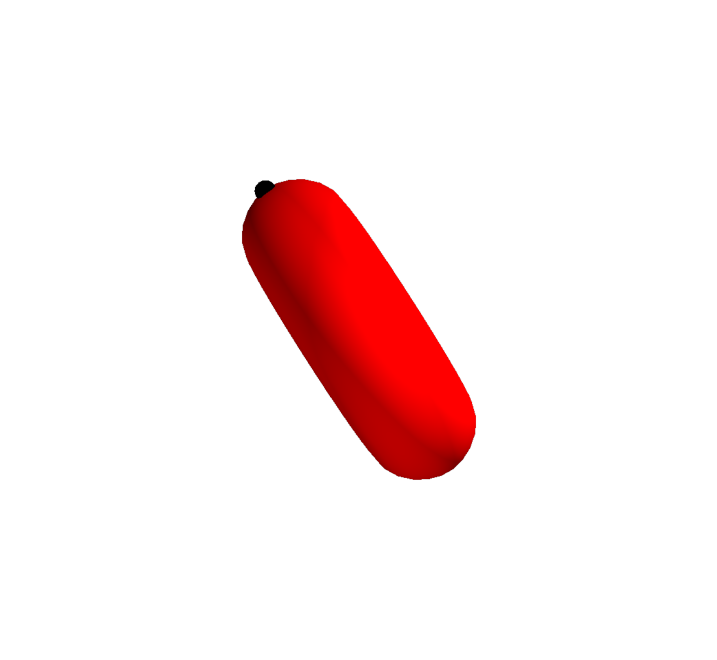
\includegraphics[trim=75 100 75 100, clip, width=\textwidth]{figures/tumble0000.png}}{0.5cm}{0.25cm}\\
        $\dot{\gamma}t = 0$
    \end{minipage}%
    \begin{minipage}{0.2\textwidth}
        \centering
        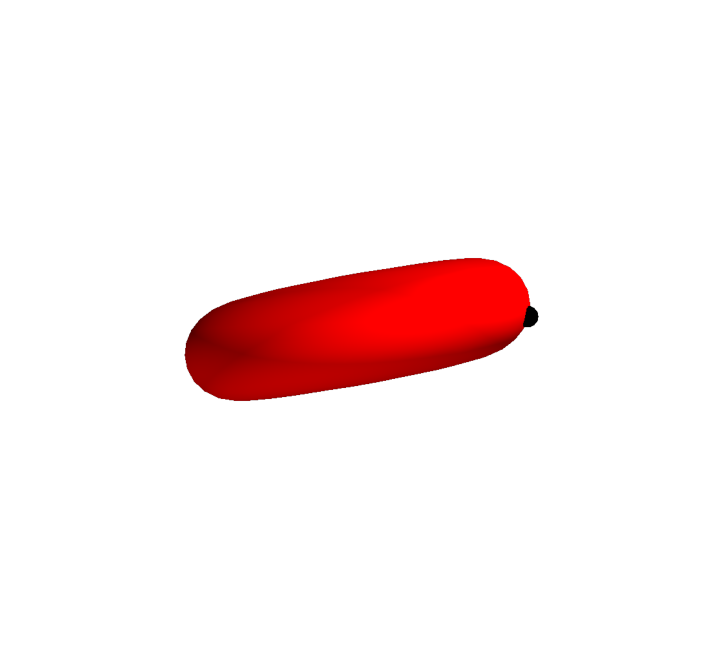
\includegraphics[trim=75 100 75 100, clip, width=\textwidth]{figures/tumble1000.png}\\
        $\dot{\gamma}t = 5$
    \end{minipage}%
    \begin{minipage}{0.2\textwidth}
        \centering
        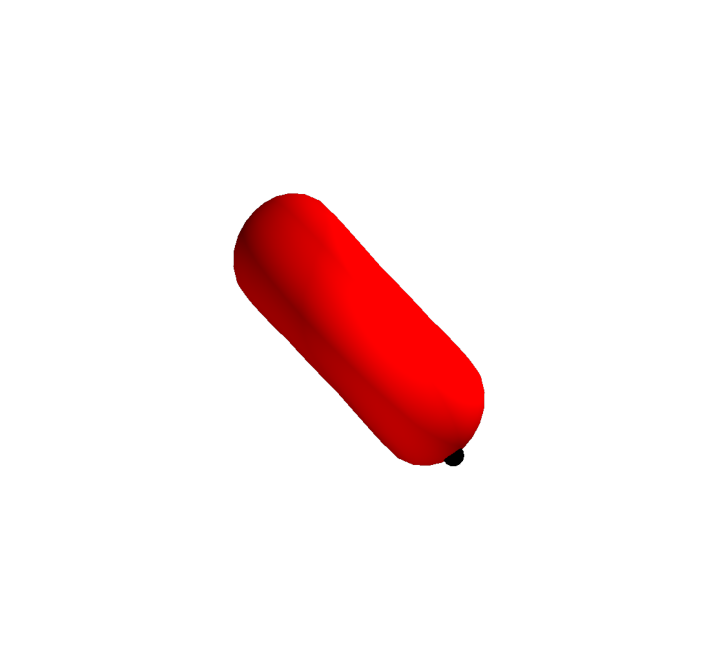
\includegraphics[trim=75 100 75 100, clip, width=\textwidth]{figures/tumble2000.png}\\
        $\dot{\gamma}t = 10$
    \end{minipage}%
    \begin{minipage}{0.2\textwidth}
        \centering
        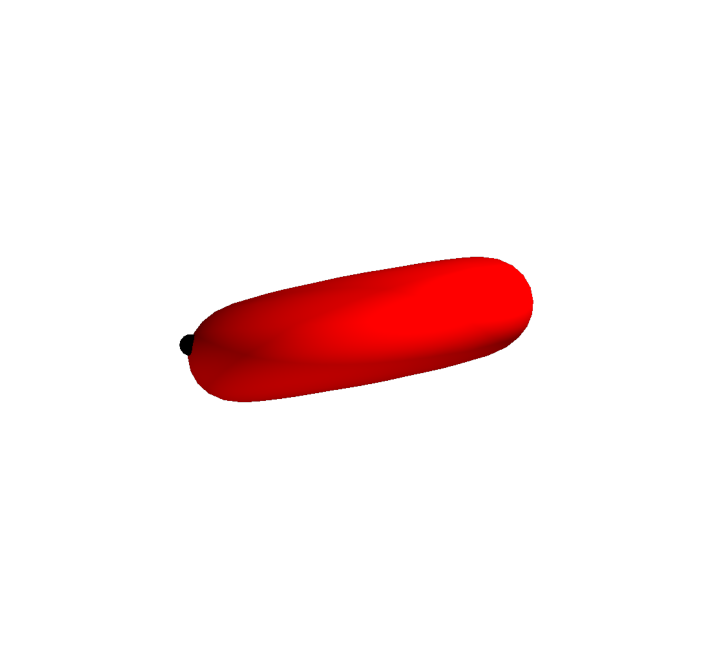
\includegraphics[trim=75 100 75 100, clip, width=\textwidth]{figures/tumble3000.png}\\
        $\dot{\gamma}t = 15$
    \end{minipage}%
    \begin{minipage}{0.2\textwidth}
        \centering
        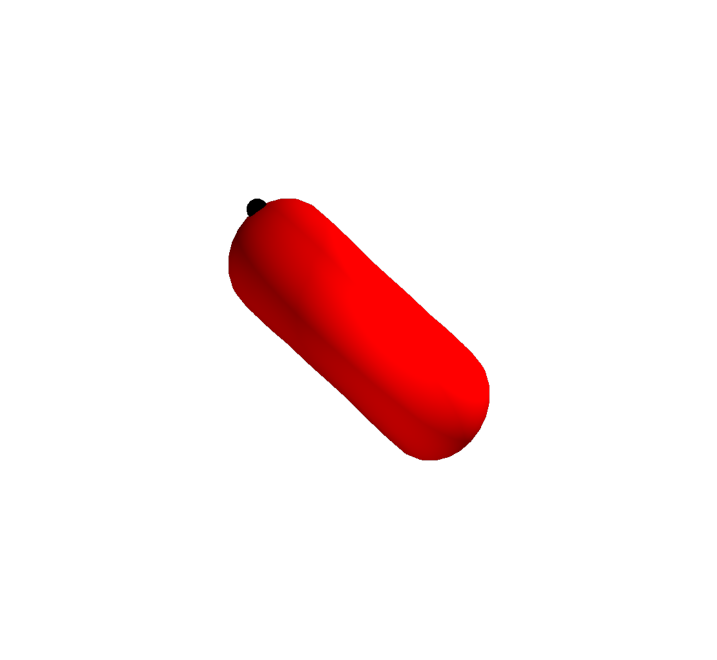
\includegraphics[trim=75 100 75 100, clip, width=\textwidth]{figures/tumble4000.png}\\
        $\dot{\gamma}t = 20$
    \end{minipage}%
    \phantomsubcaption
    \label{fig:tumble}
    \end{subfigure}
    \begin{subfigure}{\textwidth}
    \begin{minipage}{0.2\textwidth}
        \centering
        \topinset{(b)}{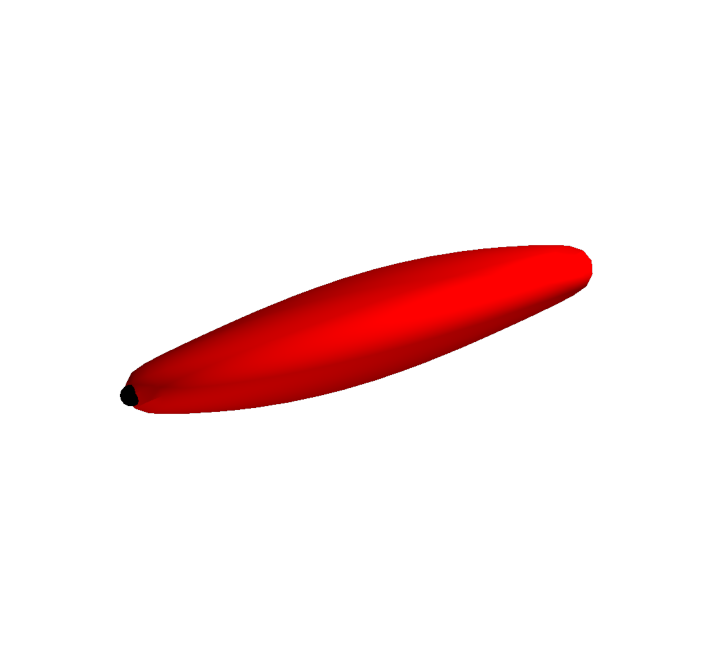
\includegraphics[trim=75 125 75 75, clip, width=\textwidth]{figures/tread0190.png}}{0.5cm}{0.25cm}\\
        $\dot{\gamma}t = 19$
    \end{minipage}%
    \begin{minipage}{0.2\textwidth}
        \centering
        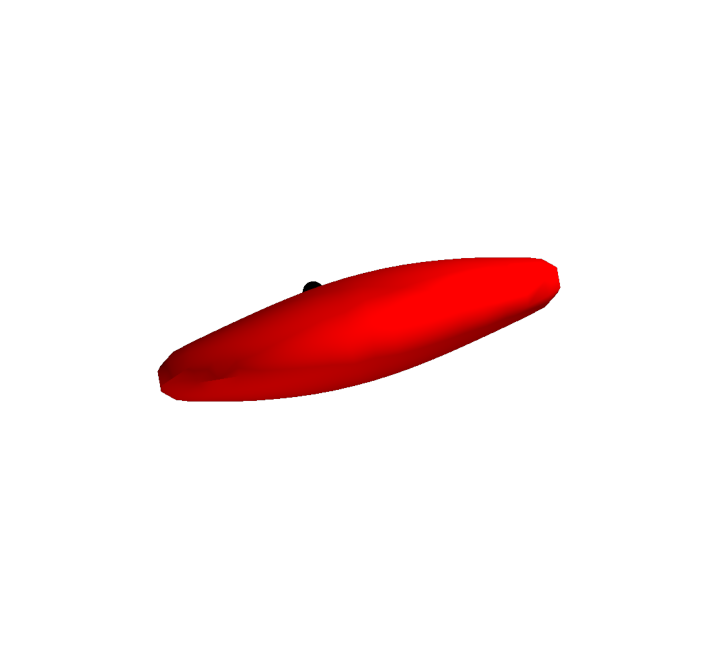
\includegraphics[trim=75 125 75 75, clip, width=\textwidth]{figures/tread0260.png}\\
        $\dot{\gamma}t = 26$
    \end{minipage}%
    \begin{minipage}{0.2\textwidth}
        \centering
        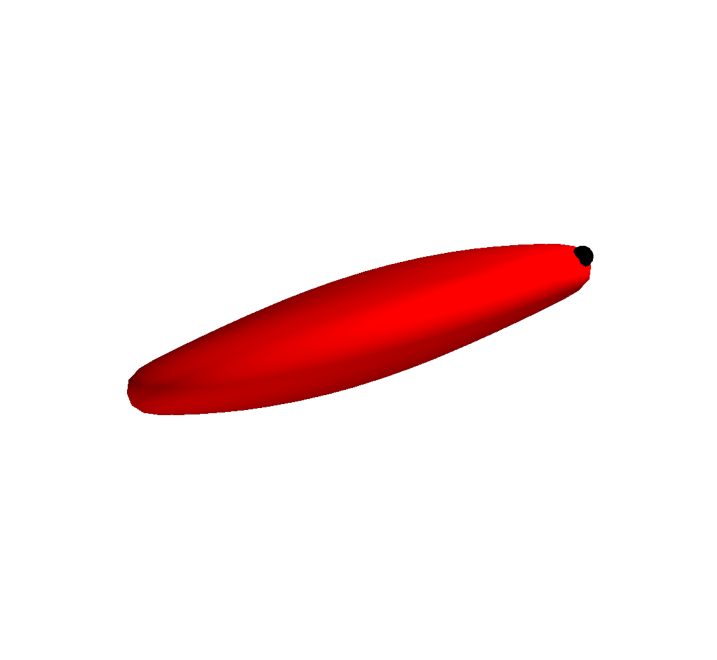
\includegraphics[trim=75 125 75 75, clip, width=\textwidth]{figures/tread0330.png}\\
        $\dot{\gamma}t = 33$
    \end{minipage}%
    \begin{minipage}{0.2\textwidth}
        \centering
        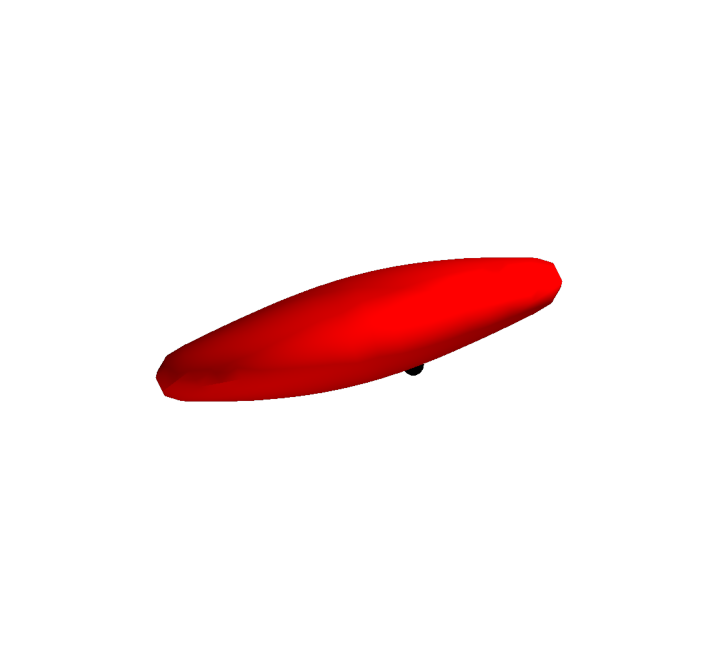
\includegraphics[trim=75 125 75 75, clip, width=\textwidth]{figures/tread0400.png}\\
        $\dot{\gamma}t = 40$
    \end{minipage}%
    \begin{minipage}{0.2\textwidth}
        \centering
        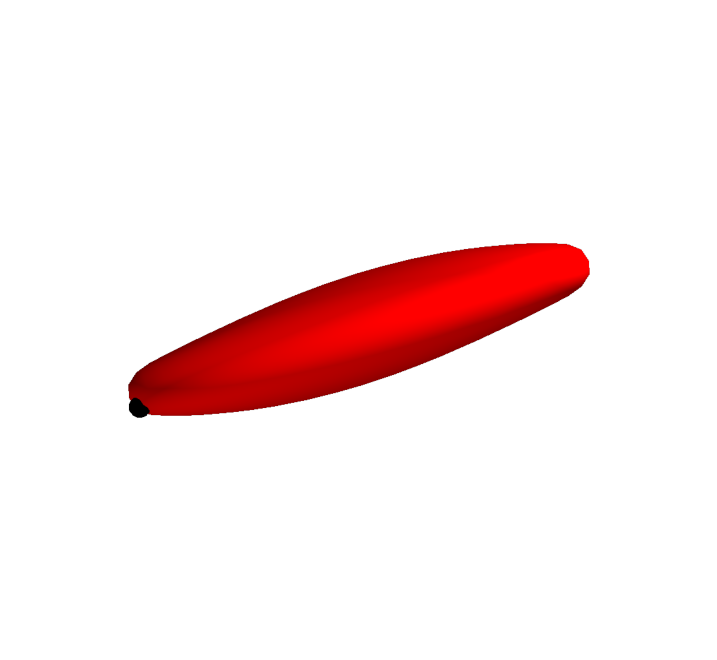
\includegraphics[trim=75 125 75 75, clip, width=\textwidth]{figures/tread0470.png}\\
        $\dot{\gamma}t = 47$
    \end{minipage}%
    \phantomsubcaption
    \label{fig:tread}
    \end{subfigure}
    \caption{%
        Our model RBC exhibits (a) a tumbling behavior under low shear
        ($\dot{\gamma} = 50\si{\per\second}$) conditions and (b) tank-treading under high
        shear ($\dot{\gamma} = 1000\si{\per\second}$) conditions.
    }%
    \label{fig:tumble-tread}
\end{figure}

%RBCs are known to tumble end-over-end under low shear conditions. As shear rates
%increase, the behavior transitions into a regime known as ``tank-treading'', in which
%the cell takes on an elongated shape and the membrane {\XXX} rotates about its interior
%fluid.
%
%We place a single RBC with $\data\cardinality = 625$ and $\sample\cardinality = 2500$
%in a $16\um\times16\um\times16\um$ domain, discretized to have $h = 0.4\um$. We use shear
%rate $\dot{\gamma} = 50\si{\per\second}$ to capture the tumbling dynamics and
%$\dot{\gamma} = 1000\si{\per\second}$ for tank-treading. One period of each is shown in
%Figure~\ref{fig:tumble-tread}.

\subsection{Collision tests}

With whole blood simulation as the ultimate goal, we must ensure that the method can effectively capture cell-cell
interactions. The RBF-IB method has been applied to flow around multiple platelets in an aggregate, but those
cells are kept apart by a network of springs~\cite{Shankar:2015km}. To study the interaction between cells, we
devise a series of tests in which we force two RBCs to collide. The aim is to verify that the cells remain
distinct. Using too few data sites could allow the cells to come too close to one another. The regularization of
$\Dirac_h$ then causes them to be treated as a single unit. Cells that ``fuse'' in this manner are problematic,
generally causing the simulation to end when the cells attempt to separate.

\begin{figure}[tb]
    \centering
    \begin{subfigure}[t]{.25\textwidth}
        \centering
        \topinset{(a)}{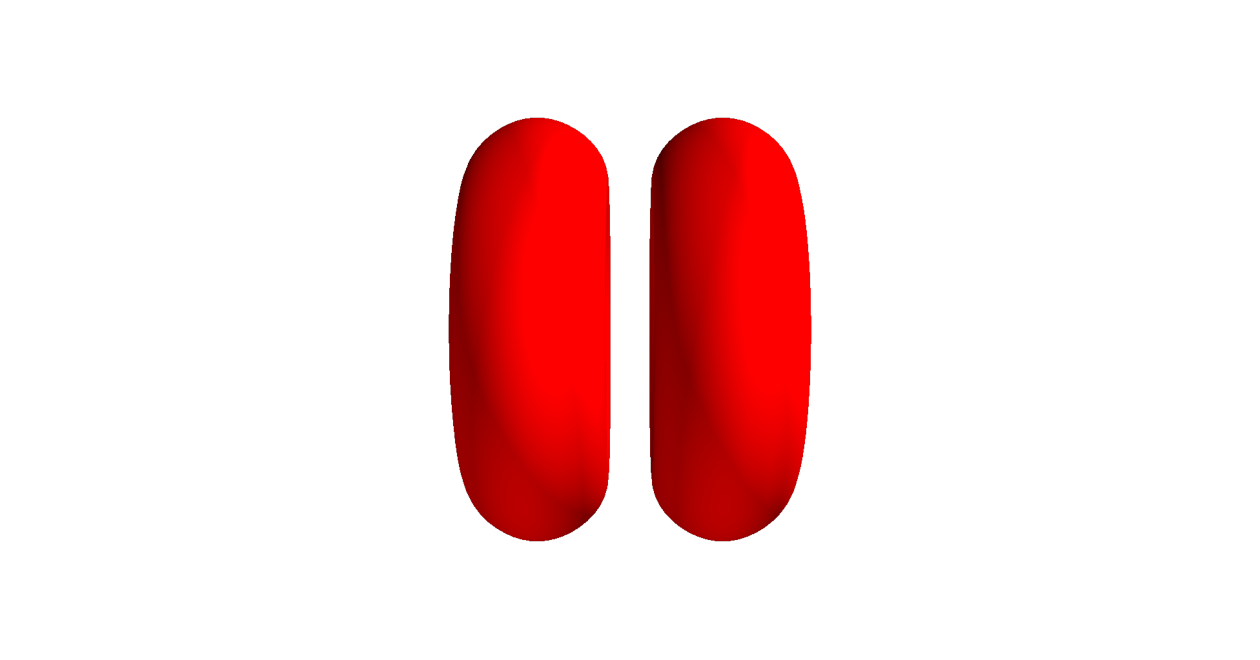
\includegraphics[width=\textwidth]{figures/vvcoll-start.png}}{0.125cm}{0.25cm} \\
        $t = 0\ms$
    \end{subfigure}%
    \begin{subfigure}[t]{.25\textwidth}
        \centering
        \topinset{(b)}{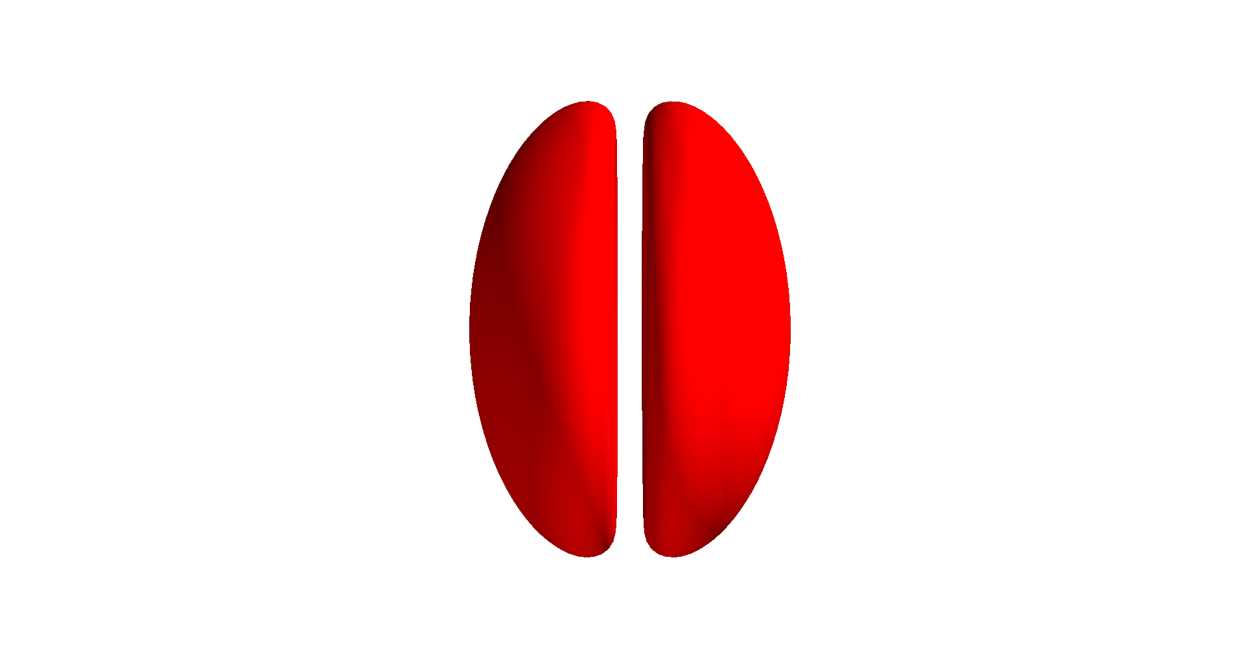
\includegraphics[width=\textwidth]{figures/vvcoll-end.png}}{0.125cm}{0.25cm} \\
        $t = 1.5\ms$
    \end{subfigure}%
    \begin{subfigure}[t]{.25\textwidth}
        \centering
        \topinset{(c)}{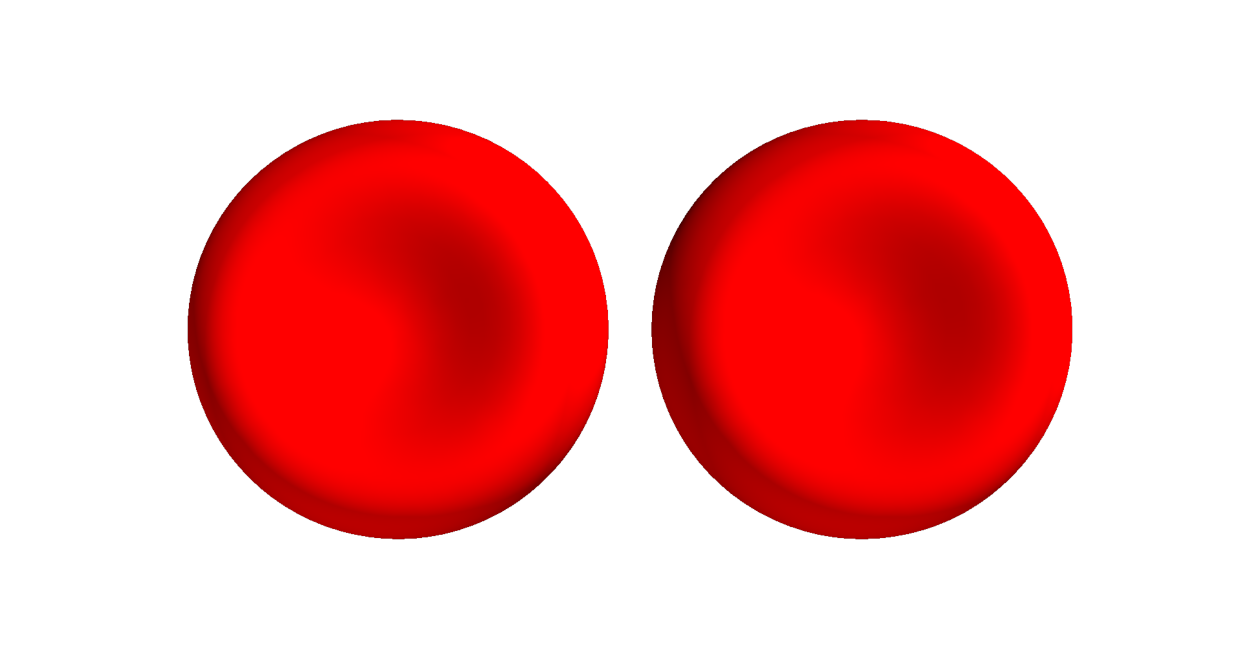
\includegraphics[width=\textwidth]{figures/hhcoll-start.png}}{0.125cm}{0.25cm} \\
        $t = 0\ms$
    \end{subfigure}%
    \begin{subfigure}[t]{.25\textwidth}
        \centering
        \topinset{(d)}{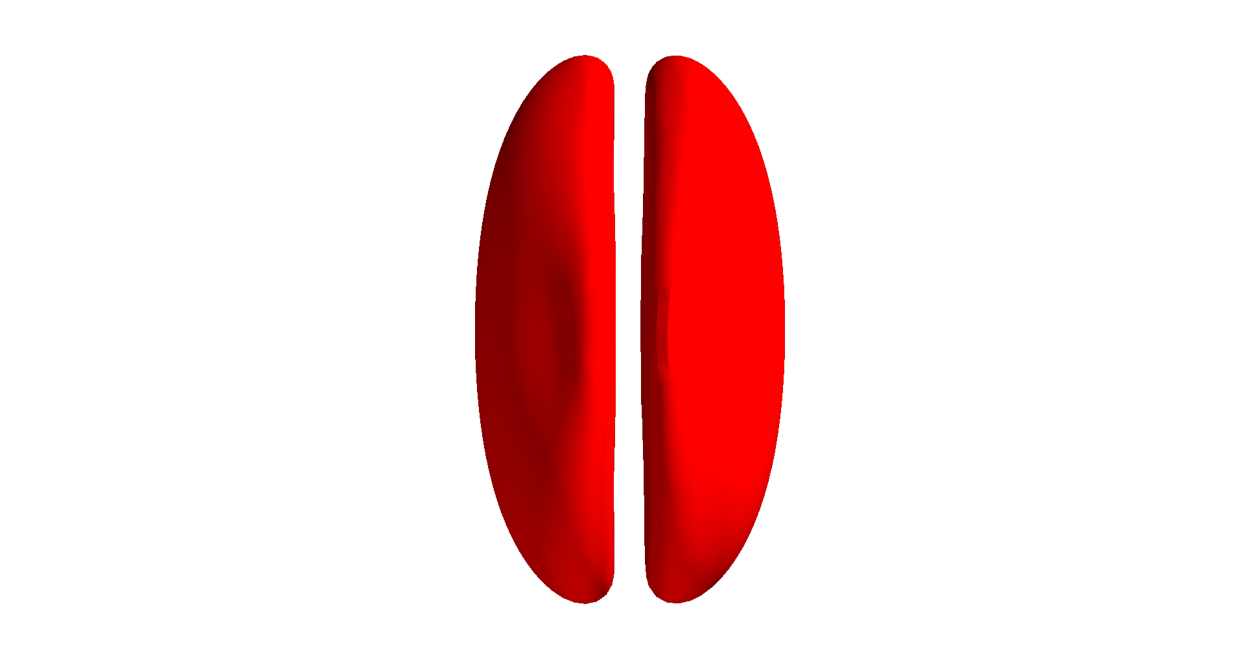
\includegraphics[width=\textwidth]{figures/hhcoll-end.png}}{0.125cm}{0.25cm} \\
        $t = 1.1\ms$
    \end{subfigure}

    \vspace{1em}

    \begin{subfigure}[t]{.25\textwidth}
        \centering
        \topinset{(e)}{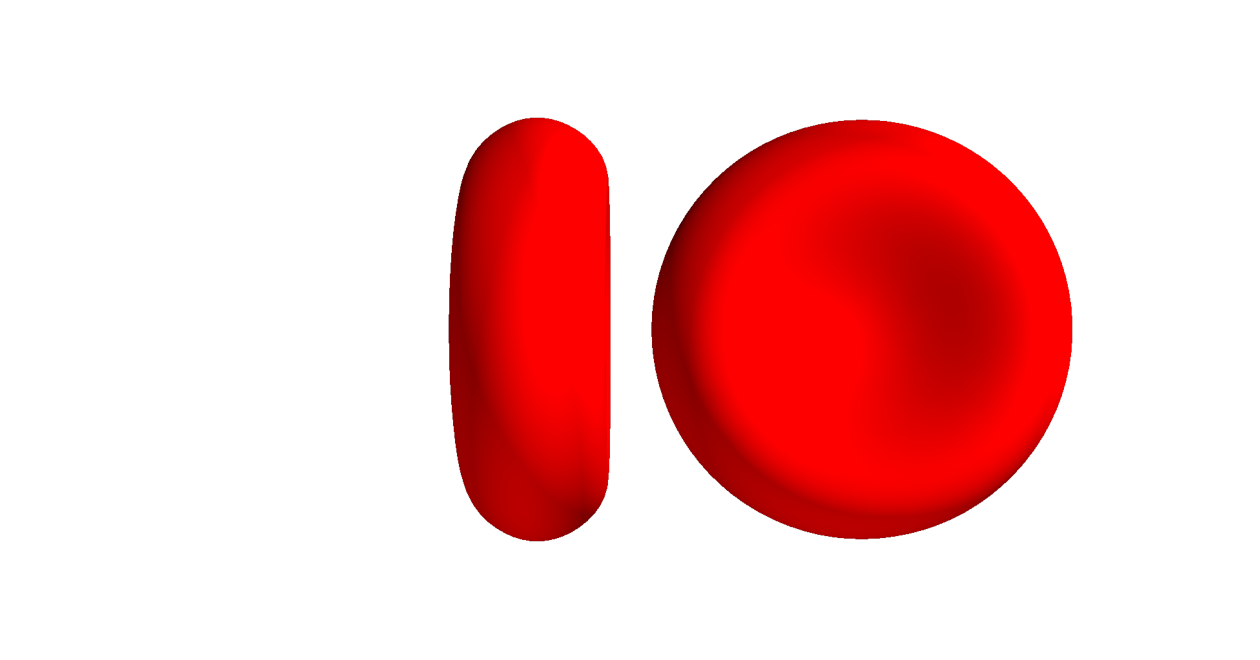
\includegraphics[width=\textwidth]{figures/vhcoll-start.png}}{0.125cm}{0.25cm} \\
        $t = 0\ms$
    \end{subfigure}%
    \begin{subfigure}[t]{.25\textwidth}
        \centering
        \topinset{(f)}{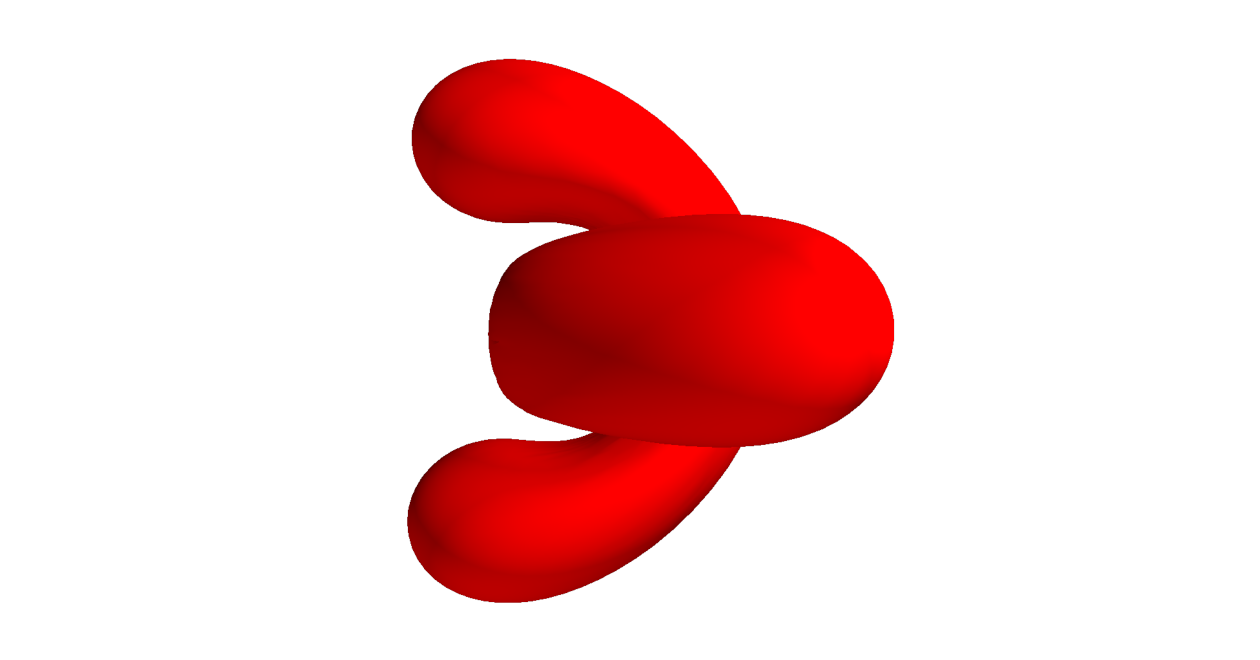
\includegraphics[width=\textwidth]{figures/vhcoll-end.png}}{0.125cm}{0.25cm} \\
        $t = 1.5\ms$
    \end{subfigure}%
    \begin{subfigure}[t]{.25\textwidth}
        \centering
        \topinset{(g)}{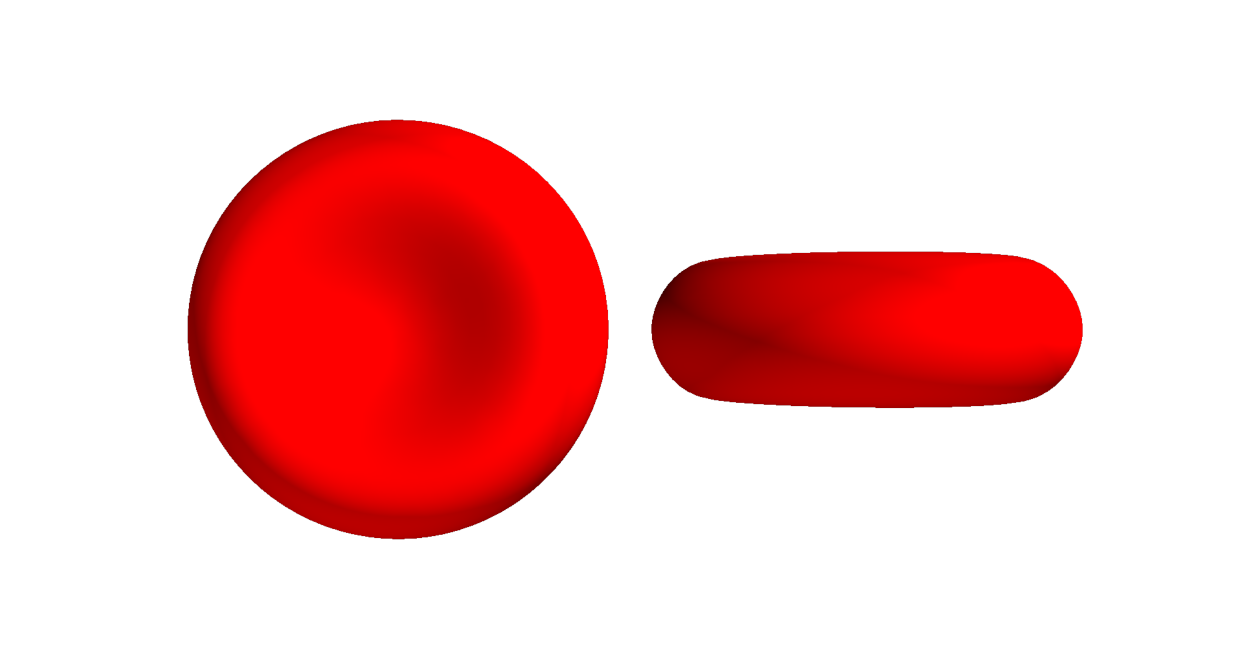
\includegraphics[width=\textwidth]{figures/rhhcoll-start.png}}{0.125cm}{0.25cm} \\
        $t = 0\ms$
    \end{subfigure}%
    \begin{subfigure}[t]{.25\textwidth}
        \centering
        \topinset{(h)}{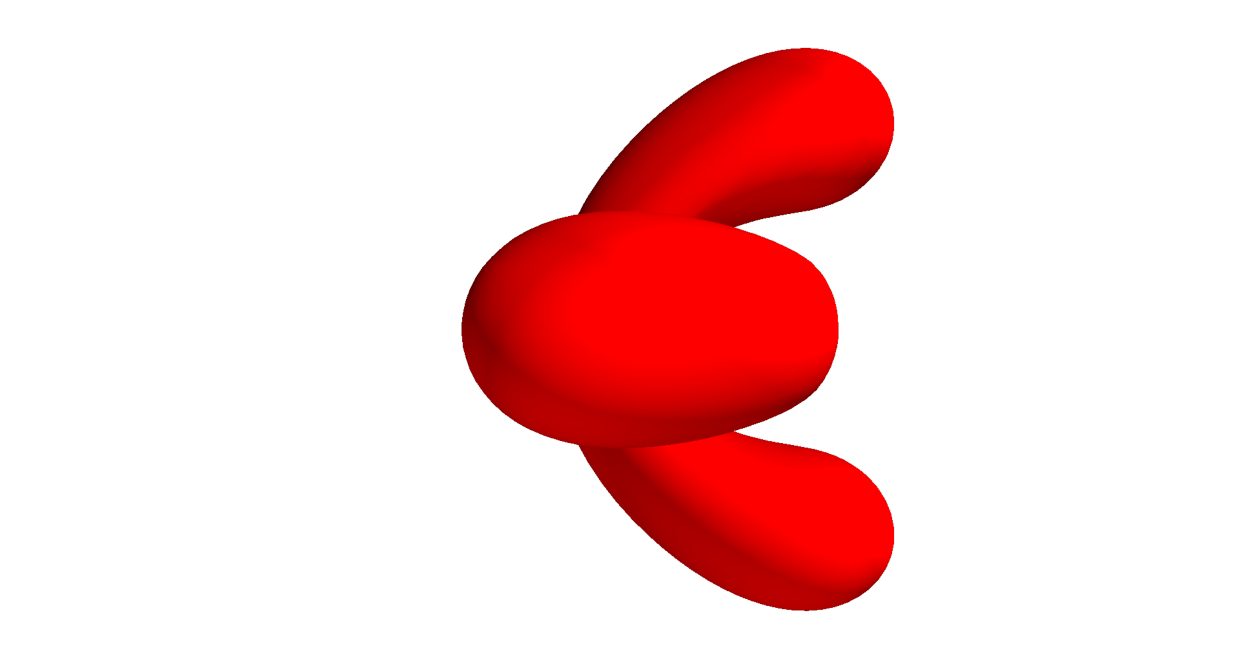
\includegraphics[width=\textwidth]{figures/rhhcoll-end.png}}{0.125cm}{0.25cm} \\
        $t = 1.1\ms$
    \end{subfigure}
    \caption{%
Collision tests between two RBCs. A fictitious force is added to the RBCs to draw them together. (a) and (b) The
RBCs are initially aligned with concavities facing one another. By $1.5\ms$, the cells take on a hemispherical
shape. The concavities in the gap are maintained. Shortly thereafter, asymmetries in the setup lead to the cells
sliding past one other. (c) and (d) The RBCs are initially aligned with their edges facing one another. By
$1.1\ms$, the cells take on a hemispherical shape. The remnants of the concavity can be seen on the left cell in
(d). Shortly thereafter, these cells also slide past one another. (e) and (f) The RBCs are initially aligned with
the edge of one facing a concavity of the other. The cells wrap around each other by $1.5\ms$, taking on a bulbous
banana shape. (g) and (h) The RBCs are initially aligned with their edges facing one another with one of the cells
rotated about the axis $\e_1+\e_3$ by $\pi/2$. By $1.1\ms$, the cells wrap around each other, again taking on the
bulbous banana shape.
    }%
    \label{fig:collisions}
\end{figure}

We continue to use the same physical domain as in the previous two sections, now with $h = 0.2\um$, and place two
RBCs therein, each with $\data\cardinality=2500$ and $\sample\cardinality=10000$. The ratio
$\sample\cardinality/\data\cardinality=4$ is chosen so that sample sites with spacing $h$ means data sites have
spacing $2h$. We believe this to suffice in preventing cells from intersecting, but this is not guaranteed if the
points do not maintain appropriate spacing throughout a simulation. We use the 2-stage RK method with time step
$\timestep = 50\ns$. To interpolate velocities and spread forces, we use the 4-point cosine $\kernel$~%
\cite{Peskin:2002go}. The cells are placed with cell centers on the line $x = z$, $y = 8\um$. They are initially
separated by a gap of $4h = 0.8\um$ between their convex hulls, \latin{i.e.}, ignoring the concavities. Inspired
by Crowl \& Fogelson~\cite{Erickson:2011cf}, we add the fictitious force density
\begin{equation}
    \F_\text{fict} = \pm 0.1\dynpercm\cdot(\e_1+\e_3)/\sqrt{2},
\end{equation}
to each cell, where the sign is chosen so the force points into the gap, to draw the cells together. Success in
these tests implies that this configuration of data and sample sites, the spatial resolution, and the time step
are acceptable for whole blood simulations.

Initial conditions and configurations after a short time are illustrated in \cref{fig:collisions}, where we view
them from above the $x=z$ plane. In each case, the cells move slightly closer together and then undergo
considerable deformation. The data sites are initially approximately $2h$ apart from each other. No problems seem
to arise from this, and in some cases the cells eventually attempt to slide past one another.  We also deduce that
the IB method with the cosine kernel can resolve interactions at a distance of $h$ to $2h$. We consider cells
passing within this threshold to be in contact. Throughout the simulation, the cells remain distinct, and the
simulations end due to extreme forces triggering the stopping condition~\cite{Agresar:1998wv}
\begin{equation}
    \timestep > \frac14\sqrt{\frac{h\rho}{\|\f\|_\infty}}.
\end{equation}
For the remainder of this chapter, we will consider only this arrangement of data and sample sites and this grid
resolution.

\subsection{Whole blood}\label{sec:whole-blood}

In what follows, we consider a $16\um\times12\um\times16\um$ domain with periodic
boundaries in the $x$ and $z$ directions and with Dirichlet boundary conditions in the
$y$ direction. The fluid velocity is initially zero except at the top boundary, where it
moves at $12\mmpersec$. In the absence of cells, the flow tends toward steady Couette
flow with a shear rate of $\shear=1000\persec$. This serves as our model near-wall region
of a blood vessel.

For whole blood simulations, we return to the 4-point B-spline, $B_3$, as the IB kernel.
Because we are limited to very small time steps with either timestepping scheme, we use
backward-forward Euler with $\timestep=50\ns$ to reduce simulation time. We observe
qualitative agreement between these two schemes.  We have already settled on an RBC
discretization in the previous section. We use the same spiral method to discretize the
platelet, but with 900 data and sample sites. Using the same number of sample sites and
data sites aligns more closely with traditional IB methods. We also find that the Bauer
spiral places points more densely along the edge of the platelet, which is helpful in
resolving the large curvatures there. We parametrize the surface of the endothelium over
$(\theta,\,\varphi) \in [0,\,2\pi)^2$ with reference shape
\begin{equation}
    \vec{\hat{X}}_\text{endo}(\theta,\,\varphi) = \left[\begin{array}{c}
            16\um\cdot(\theta/2\pi)  \\
            y(\theta,\,\varphi) \\
            16\um\cdot(\varphi/2\pi)
    \end{array}\right],
\end{equation}
where $y(\theta,\,\varphi)$ depends on the shape under study. The endothelium is
discretized using 16000 points, defined by the spiral
\begin{align*}
    \varphi_i &= 2\pi (i-1)/N, \\
    \theta_i &= \modulo\left(\left\lceil\!\sqrt{N}\mskip\thinmuskip\right\rceil\varphi_i,\,2\pi\right).
\end{align*}
We consider two shapes for the endothelium. The first, $y=1\um$, emulates the flat wall
typically seen in near-wall simulations of RBCs or platelets. The other attempts to
recreate the elongated endothelial cell shape typical of exposure to high-shear
conditions,
\begin{equation*}
    y(\theta,\,\varphi) = 0.75\um + 1\um\cdot\cos^2(\theta-\varphi)\sin^2(\varphi/2).
\end{equation*}
The bumps have a prominence of $1\um$. The endothelial surface is raised by $0.75\um$ to
avoid it interacting with the domain boundary. The positions of the surface are chosen to
maintain a fixed hematocrit of approximately 34\% for both endothelial shapes.

As a preliminary validation of the platelet model and to establish baseline platelet
motion, we consider two platelets along a flat wall. They are placed parallel to the wall
at distances of $0.3\um$ and $0.5\um$. The domain does not contain any RBCs. At a
distance of $0.3\um$, the platelet is expected to ``wobble'', in which the platelet tilts
slightly upward and downward, periodically~\cite{King:2005fv}. On the other hand, the
platelet initially $0.5\um$ from the wall should tumble end-over-end $0.5\um$. We observe
wobbling at a frequency of approximately $10\persec$ and tumbling with a frequency of
approximately $30\persec$. We also note that the edge of the tumbling platelet remains
pointed towards the wall for only 3--$4\ms$.

\subsubsection{Initialization}\label{sec:blood-init}

We begin by assuming that the platelets have already been marginated by the RBCs. We
think of the domain as having three layers with the endothelium at the bottom, RBCs on
top, and platelets in between. We begin by settling the endothelium and RBCs before
placing platelets.

In addition to the endothelium, we place 2 rows of 4 RBCs, each in their reference
configuration, in the domain with the RBCs' centers of mass on the plane $y=6\um$.
Because the domain is not wide enough to accommodate two reference RBCs alongside one
another, the cells are staggered by $2\um$. These locations are then randomly translated
and rotated while maintaining a distance of at least $2h$ between cells.

Before placing any platelets in the domain, we allow the flow to develop with only the
endothelium and RBCs. We allow the initialization to continue until at least $17\ms$,
which is approximately when the first RBC overtakes its neighbor. From here, we choose a
series of times, sampled from a Poisson distribution to be approximately $3\ms$ apart, at
which to begin simulations with platelets.

The RBCs for each of the chosen starting configurations are considerably and
unpredictably deformed and have left a space of a few microns above the endothelium
in which we place platelets. To find reasonable starting orientations for the platelets,
we randomly choose points on the endothelium and one on each platelet surface. Each of
the simulations in the upcoming sections contains two platelets, so we choose two points
on the endothelium that are at least $3.9\um$, a platelet diameter plus $4h$, apart. The
resulting platelet are spaced far enough apart as to not intersect. We compute normal
vectors on the surfaces of the endothelium and platelets at these points. The platelets
are oriented so that the normal emanating from the platelet opposes the normal at the
corresponding point on the endothelium. The platelet is then placed so its chosen surface
point is separated from the endothelium point by a random distance between $0.3\um$ and
$1\um$. If the generated orientation does not pass within $0.4\um$ of an RBC, the
platelet is accepted. Otherwise, we try again with a different platelet point. This
algorithm typically succeeds within 2 attempts.

This initialization process is performed once for each endothelial configuration and we
take the first four acceptable initial configurations for each. In the following section,
we present behaviors found in these simulations. As a point of comparison, we also
consider the initial configurations for the bumpy wall with the RBCs removed from the
domain.


\subsubsection{Characterization of flow and cell behaviors}

In this section, we catalog the differences in the flow between whole blood along a bumpy
and flat wall, and between flow along a bumpy wall with and without RBCs. We aim to
compare the interactions platelets have with RBCs and the endothelium for these test
cases.
%We begin with the expected behaviors before moving on to remarkable ones.

\begin{figure}[tp!]
    \centering
    \begin{tikzpicture}[spy using outlines={rectangle, magnification=3,connect spies}]
        \begin{axis}[
                axis lines=center,
                xmin=0,
                xmax=12.5,
                ymin=0,
                ymax=12.5,
                ylabel={$y$ ($\um$)},
                xlabel={fluid speed ($\mmpersec$)},
                xlabel near ticks,
                ylabel near ticks,
                legend pos=south east,
                legend style={draw=none}
            ]
            \addplot[color=tol/contrast/red, very thick, x filter/.code={\pgfmathparse{\pgfmathresult*10}\pgfmathresult}] table [x index=1, y index=0] {rpefast1.prof.dat};
            \addlegendentry{\cmark~bumps\hspace{0.5em}\cmark~RBCs};
            \addplot[color=tol/contrast/blue, very thick, x filter/.code={\pgfmathparse{\pgfmathresult*10}\pgfmathresult}] table [x index=1, y index=0] {rpeflat1.prof.dat};
            \addlegendentry{\xmark~bumps\hspace{0.5em}\cmark~RBCs};
            \addplot[color=tol/contrast/yellow, very thick, x filter/.code={\pgfmathparse{\pgfmathresult*10}\pgfmathresult}] table [x index=1, y index=0] {pefast1.prof.dat};
            \addlegendentry{\cmark~bumps\hspace{0.5em}\xmark~RBCs};

            \coordinate (spypoint) at (axis cs: 0.5, 1);
            \coordinate (spyviewer) at (axis cs: 2.5, 10);
            \spy[width=2cm,height=2cm] on (spypoint) in node [fill=white] at (spyviewer);
        \end{axis}
    \end{tikzpicture}
    \caption[A comparison of fluid velocity profiles]{%
Time- and space-averaged fluid velocity profiles for each of the test cases.
%The F\r{a}hr{\ae}us-Lindqvist effect is clearly evident when RBCs are included.
The inclusion of RBCs (red and blue curves) causes the region inhabited by platelets,
1--$4\um$, to experience a higher shear rate than it would without RBCs (yellow curve).
    }\label{fig:flow-profiles}
\end{figure}

Flow profiles are shown in Figure~\ref{fig:flow-profiles}. The most notable difference
among the three flow profiles is the nearly Couette flow when RBCs are absent. The only
distinction between this and Couette flow is the smoother transition at the wall, due to
the bumps. This is also the distinguishing feature between the profiles corresponding to
bumpy and flat walls in the presence of RBCs. The smooth transition from the bumps
results in marginally slower flow speeds throughout the domain, compared to the flat
wall. The inclusion of RBCs causes the bends in the red and blue curves around $y = 3\um$
and $y = 9\um$. Platelets inhabit the region between $y=1$ and $3\um$. In simulations
featuring RBCs, the platelets experience higher shear rates than those without RBCs where
there is a reduction in apparent viscosity in the RBC-free layer. This is a consequence
of the F\r{a}hr{\ae}us effect. In pressure-driven flow through a tube, we expect
approximately parabolic flow.  The bend near $y = 9\um$ is therefore nonphysical and
arises from satisfying boundary conditions at the top boundary. However, the increased
shear rate in the region between $y=9$ and $12\um$ seems to be useful in deterring RBCs
from approaching the upper boundary. An exclusionary region of just 1--$2\um$ along the
top boundary increases the effective hematocrit to 37--41\%. Furthermore, the reduced
shear rate in the region containing RBCs results in slower tank-treading compared to a
dilute suspension of RBCs, with one period now lasting approximately $40\ms$.

RBCs are effective at preventing the platelets from moving too far from the endothelium.
The furthest observed distance from the endothelium any platelet takes is just under
$1.5\um$. Likewise, RBCs infrequently enter the cell-free layer, with some notable
exceptions, discussed below. We do not observe any platelet wobbling. Instead, platelets
transiently follow the curve of the bumpy walls, tilt down into the valleys between
bumps, and tumble. Nothing suggests that bumps in the surface of the endothelium alone
can sequester platelets, nor do we directly observe stagnation zones.

\begin{figure}[th!]
    \begin{subfigure}[t]{0.5\textwidth}
        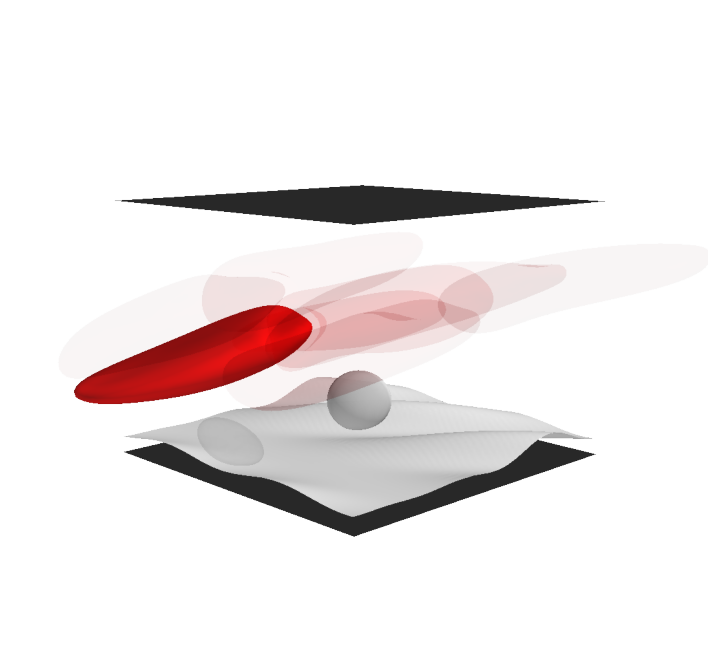
\includegraphics[trim=50 75 50 125, clip, width=\textwidth]{figures/unicycle1.png}
        \subcaption{$t = 46\ms$}
    \end{subfigure}%
    \begin{subfigure}[t]{0.5\textwidth}
        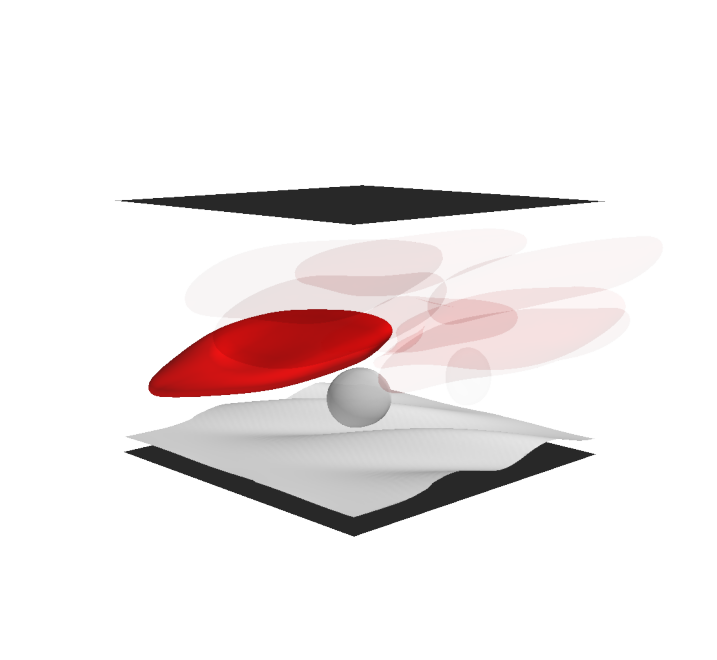
\includegraphics[trim=50 75 50 125, clip, width=\textwidth]{figures/unicycle2.png}
        \subcaption{$t = 48\ms$}
    \end{subfigure}

    \vspace{11pt}

    \begin{subfigure}[t]{0.5\textwidth}
        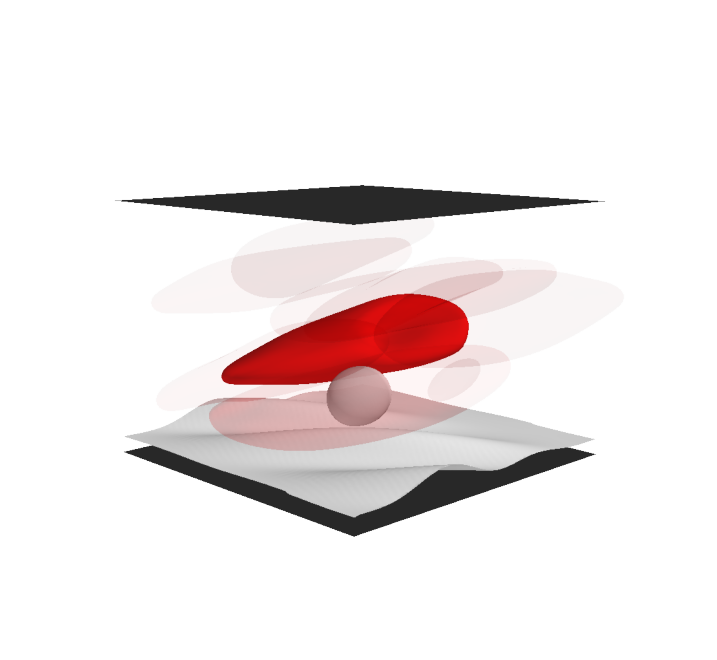
\includegraphics[trim=50 75 50 125, clip, width=\textwidth]{figures/unicycle3.png}%
        \subcaption{$t = 50\ms$}
    \end{subfigure}%
    \begin{subfigure}[t]{0.5\textwidth}
        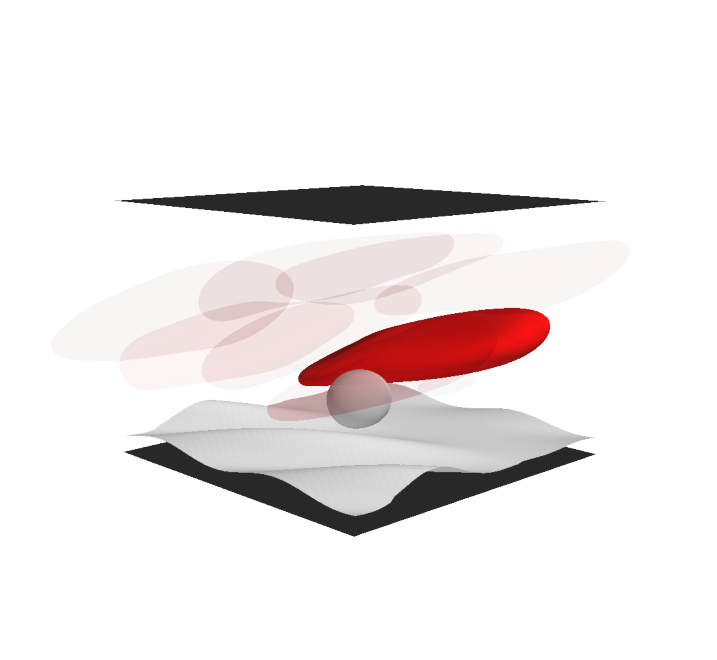
\includegraphics[trim=50 75 50 125, clip, width=\textwidth]{figures/unicycle4.png}%
        \subcaption{$t = 52\ms$}
    \end{subfigure}

    \vspace{11pt}

    \begin{subfigure}[t]{\textwidth}
        \begin{tikzpicture}
            \begin{axis}[
                width=\textwidth,
                height=2in,
                axis lines=center,
                xmin=8.5,
                xmax=61.5,
                ymin=0,
                ymax=0.95,
                ylabel={distance ($\um$)},
                xlabel={time ($\ms$)},
                xlabel near ticks,
                ylabel near ticks
            ]
                \addplot[color=tol/vibrant/magenta, very thick] table [x index=0, y index=6] {rpefast0.dat};
                \addplot[no marks, color=black, dashed] coordinates {(8.5, 0.4)
                                      (61.5, 0.4)};
                \path[name path=axis] (axis cs: 8.5, 0) -- (axis cs: 61.5, 0);
                \addplot[opacity=0, name path=unicycle] table [x index=0, y index=4] {rpefast0.dat};
                \addplot[fill=tol/vibrant/magenta, fill opacity=0.2] fill between[of=unicycle and axis];

                \node at (axis cs: 10.5, 0.9) {(e)};
            \end{axis}
        \end{tikzpicture}
    \end{subfigure}
    \caption[Platelet unicycling behavior]{%
(a)--(d) Snapshots of a platelet rolling on its edge (``unicycling'') with RBCs, one
translucent, flanking either side. The camera tracks the opaque platelet. It's motion is
indicated by the endothelium moving from right to left. (e) The distance between
the platelet and the endothelium. The shaded region indicates that the orientation of the
platelet's short axis is within $45^\circ$ of the vorticity direction.  The black dashed
line indicates $2h$ and is the maximum distance that might be considered contact with the
endothelium. See~\ref{sec:supp} for a video corresponding to this simulation.
    }\label{fig:unicycle}
\end{figure}

Bumpy endothelium simulations without RBCs mimic those with a flat wall; platelets move
away from the wall to a point where they are free to tumble. Unsurprisingly, we observe
platelet tumbling for both flat and bumpy walls with RBCs as well. In Stokes-like flow, a
rigid platelet would tumble faster in flow with a higher shear rate. We might therefore
expect the platelet to tumble faster with RBCs. However, RBCs can significantly disturb
the fluid around a platelet, speeding up its motion, slowing it down, or preventing a
tumble altogether.

We observe platelets rolling in the flow direction along their edge. Because the
platelet in this arrangement is aligned vertically, part of the edge stays in
near-contact with the endothelium while the opposite edge extends into the region
occupied by RBCs.  Contact with RBCs is frequent. These contacts can have a destabilizing
effect, but may also prolong the rolling. Figure~\ref{fig:unicycle}(a)--(d) consists of a
series of snapshots illustrating the behavior. The platelet in this case is flanked by
two RBCs, so it does not have the space to topple over until the RBCs pass a few
milliseconds later.

While Figure~\ref{fig:unicycle} shows this phenomenon on a bumpy wall, it can also occur
above a flat wall. We first observed this motion with a flat wall, and there it lasted
over $40\ms$. The motion was maintained, in part, by an RBC that rode along the top of
the platelet, partially enveloping that platelet. We say that a platelet rolling on its
edge is \term{unicycling}. Figure~\ref{fig:unicycle}(e) illustrates that the platelet
spends more time in contact or near-contact with the endothelium while unicycling
compared to the tumbles near $t=16\ms$ and $t=29\ms$. Though RBCs seem to control the
duration of the unicycling, they are not strictly necessary for unicycling to occur. In
tests with a bumpy wall without RBCs, unicycling is initiated when a platelet rolls
sideways, relative to the flow direction, off of a bump. Without RBCs, the platelet
maintains the vertical alignment for a majority of the simulation thereafter. However,
without frequent interaction with RBCs, the platelet in these simulations move away from
the wall.  Moreover, while we have not observed it directly, we expect that a lone
platelet traveling over a flat wall would also exhibit unicycling, given the right
initial orientation.

\begin{figure}[th!]
    \begin{subfigure}[t]{0.5\textwidth}
        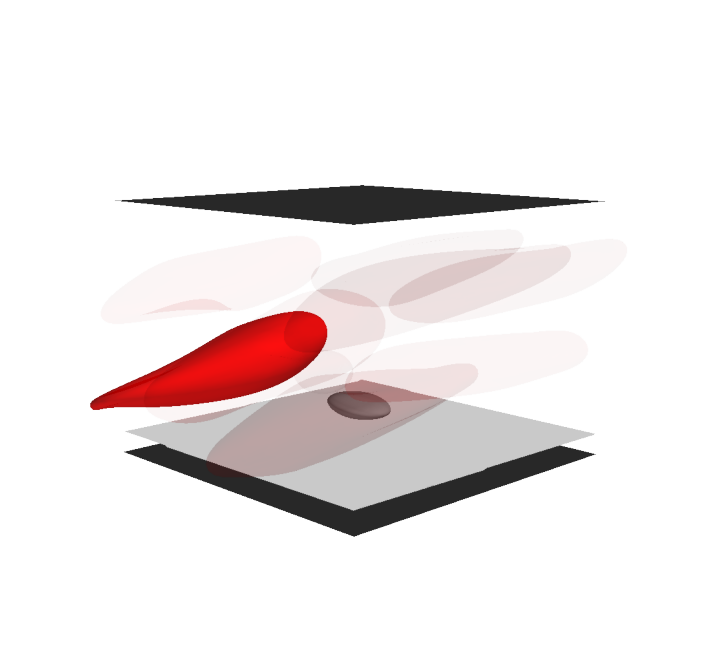
\includegraphics[trim=50 75 50 125, clip, width=\textwidth]{figures/flyover460.png}%
        \subcaption{$t = 46.0\ms$}
    \end{subfigure}%
    \begin{subfigure}[t]{0.5\textwidth}
        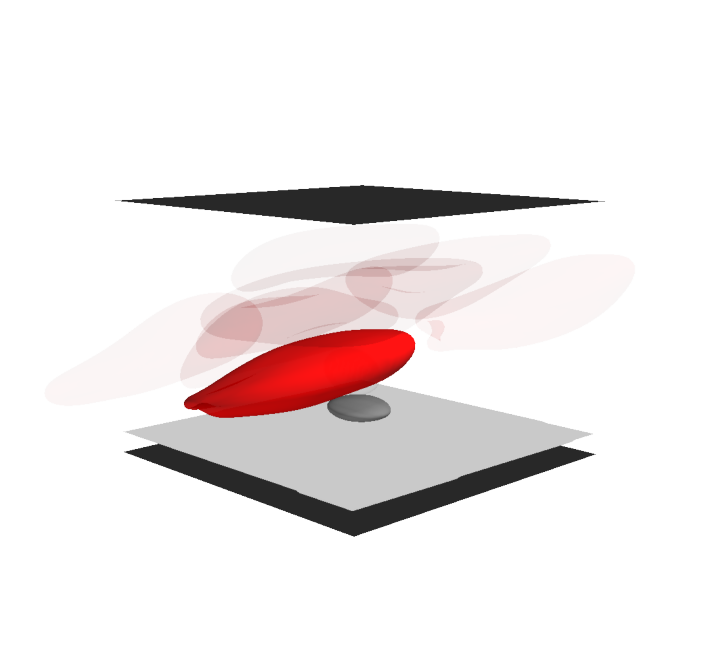
\includegraphics[trim=50 75 50 125, clip, width=\textwidth]{figures/flyover495.png}
        \subcaption{$t = 49.5\ms$}
    \end{subfigure}

    \vspace{11pt}

    \begin{subfigure}[t]{0.5\textwidth}
        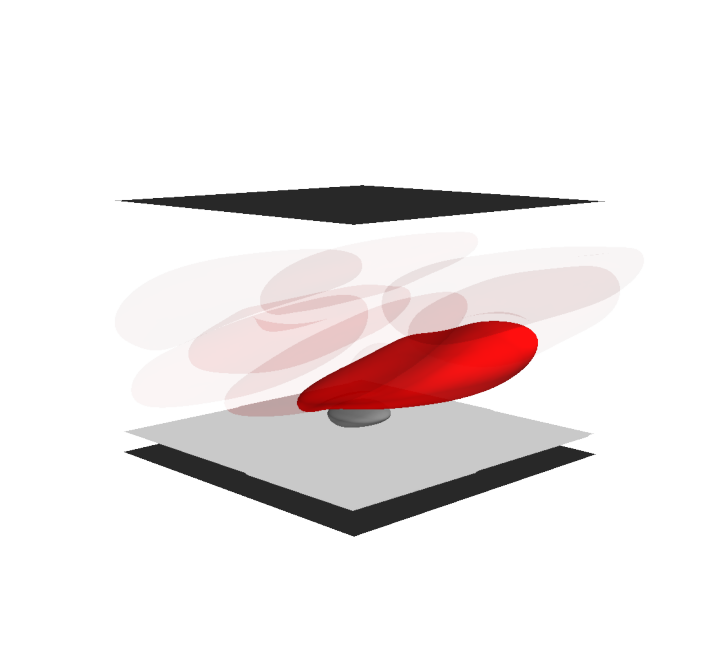
\includegraphics[trim=50 75 50 125, clip, width=\textwidth]{figures/flyover530.png}%
        \subcaption{$t = 53.0\ms$}
    \end{subfigure}%
    \begin{subfigure}[t]{0.5\textwidth}
        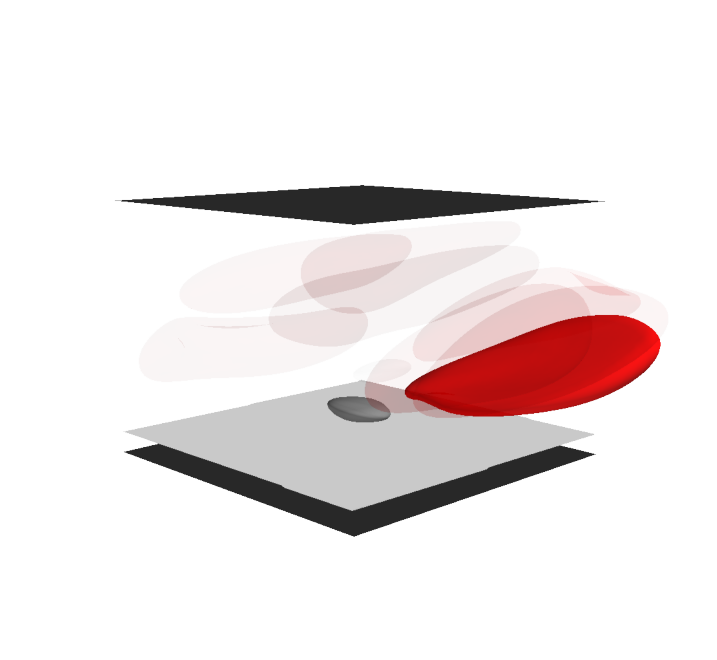
\includegraphics[trim=50 75 50 125, clip, width=\textwidth]{figures/flyover565.png}%
        \subcaption{$t = 56.5\ms$}
    \end{subfigure}

    \vspace{11pt}

    \begin{subfigure}[t]{\textwidth}
        \begin{tikzpicture}
            \begin{axis}[
                width=\textwidth,
                height=2in,
                axis lines=center,
                xmin=8.5,
                xmax=61.5,
                ymin=0,
                ymax=3.25,
                ylabel={velocity ($\mmpersec$)},
                xlabel={time ($\ms$)},
                xlabel near ticks,
                ylabel near ticks
            ]
                \addplot[color=tol/vibrant/magenta, very thick] table [x index=0, y index=3] {rpeflat3.vel.dat};
                \path[name path=axis] (axis cs: 8.5, 0) -- (axis cs: 61.5, 0);
                \addplot[opacity=0, name path=deformed, y filter/.code={\pgfmathparse{#1*3}\pgfmathresult}] table [x index=0, y index=4] {rpeflat3.vel.dat};
                \addplot[fill=tol/vibrant/magenta, fill opacity=0.2] fill between[of=deformed and axis];

                \node at (axis cs: 10.5, 3) {(e)};
            \end{axis}
        \end{tikzpicture}
    \end{subfigure}
    \caption[RBC-mediated platelet-endothelial collision]{%
(a)--(d) Snapshots of RBC-mediated collision between a platelet and the endothelium. (a)
The platelet attempts to tumble. (b)--(c) An RBC comes into proximity with the platelet,
deflects to avoid the platelet, and pushes the platelet into the endothelium, thereby
preventing the platelet from tumbling. (d) The platelet is free to tumble again. (e) The
minimum velocity on the surface of the platelet. The shaded region indicates that the
relative change in aspect ratio exceeds 4\%. See~\ref{sec:supp} for a video corresponding
to this simulation.
    }\label{fig:rbc-plt-endo-collision}
\end{figure}

We notice that in simulations with a bumpy endothelium, platelets will collide with the
bumps. This tends to occur while the platelet is tumbling, and the edge of the platelet
makes contact with the endothelium. This interaction is characterized by deformations
that flatten the edge of the platelet and a \midtilde5\% relative
change in the aspect ratio of the platelet. However, the collision need not occur along
the edge of the platelet, nor, indeed, against a bump in the endothelium. Similar
collisions occur in the case of a flat wall, suggesting that RBCs mediate this behavior.
A clear case of this is illustrated in Figure~\ref{fig:rbc-plt-endo-collision}(a)--(d).
We also note that the few milliseconds preceding the unicycling in Figure~%
\ref{fig:unicycle} correspond to a collision with the wall, showing that this is yet
another trigger for unicycling to occur.

Because the platelet comes into contact with the endothelium, or nearly does so, the
platelet slows along the area of contact. Figure~\ref{fig:rbc-plt-endo-collision}(e)
shows the correlation between the relative change in aspect ratio and the reduction in
minimum platelet surface velocity. Though the aspect ratio of the platelet changes
somewhat while normally tumbling, changes of this magnitude seem to always correspond to
interactions with the endothelium. Collisions with the RBC, for example, result primarily
in deformation of the RBC and deflection of the platelet, which is otherwise relatively
unperturbed.


\section{Discussion}\label{sec:conclusion}

In this article, we developed a coherent numerical framework based on the RBF-IB method for whole blood
simulation. We have shown that a continuous energy RBF-based model RBC incorporating dissipative forces exhibits
the traditional tumbling and tank-treading behaviors. We simulated the flow of whole blood involving RBCs and
platelets over a model endothelium. We considered both flat and bumpy endothelial shapes and flow with and without
RBCs along a bumpy wall.

The most prominent result of the whole blood simulations is that simulations involving platelets but neglecting
the influence of RBCs cannot capture the true nature of platelet motion. In fact, platelets near the endothelium
experience augmented shear rates due to RBCs and RBCs act to confine platelets to the cell-free layer. Simulations
without RBCs fail to capture the more irregular aspects of platelet motion. In fact, our simulations show that
interaction with RBCs can disturb otherwise regular wobbling motions exhibited by platelets, and also appear to
delay tumbling. Our results also demonstrate that certain platelet behaviors can only be observed by considering
numerous starting configurations in developed flows involving RBCs.

Another prominent finding is that the effect of RBCs generally overwhelms the effects of the wall topography.
\Cref{fig:flow-profiles} shows that the flat wall yields slightly faster fluid velocities, but the flow profiles
for flat and bumpy walls are qualitatively the same, except for the immediate vicinity of the wall. The result is
a region of space between the bumps with a velocity gradient. Platelets following the shape of the bumpy wall
crest the bump, dip into the region of lower velocity, and tumble. This feature is absent from the flat wall, but
tumbling is not an extraordinary behavior. In either case, we observe ``unicycling\qend,'' a unique behavior in
which the platelet rolls in the flow direction along its edge. Unicycling can be stabilized by RBCs which flank
the platelet, or by an RBC that partially encapsulates the platelet while passing over it. Conversely, it can also
be destabilized by an RBC passing on one side. The endothelial protrusions are also sufficient to orient a platelet
while unicycling, but without RBCs to confine the platelet near the wall, the platelet does not roll along the
wall for long. However, we find that unicycling itself seems to be stable. Unicycling also highlights the need for
3D simulations---it is a behavior that cannot be captured by or predicted from a 2D simulation. We also observe
platelet-endothelial interactions for both endothelial shapes. These interactions are typically caused by RBCs
driving the platelet into the endothelium. The collisions are characterized by significant deformation to the
platelet and a reduction in its speed. From a qualitative standpoint, the endothelial shape alone has minimal
impact on the motion of the platelets, meaning that for modeling flow of whole blood above a healthy blood vessel, a flat wall suffices.

It is also reasonable to consider an alternative interpretation of the flat wall: a model exposed subendothelium.
Near contact with the subendothelium increases the chance of platelet activation.  Unicycling keeps an edge of the
platelet near the wall, without hindering mobility. We see that the vertical alignment is often maintained much
longer than wall contacts from tumbling, and we do not observe wobbling in the presence of RBCs.  We propose
unicycling as an effective means by which platelets survey the vasculature for injury. Of course, the platelet can
only distinguish a healthy vessel from an injury by encountering the necessary chemical signals. Until then, the
platelets unicycle around bumps along the healthy endothelium as well. This also implies that unicycling
indirectly assists in platelet activation for these shear rates.

We also consider yet another alternative interpretation of the bumpy wall. Because the bumps are approximately the
same size as a platelet, we can consider this to be a rough model of a subendothelium with a few deposited
platelets. Under this interpretation, we view platelet-wall contact as interactions between an unactivated
platelet and the subendothelium, when contact occurs in a valley, or between an unactivated platelet and an
activated platelet adhering to the subendothelium, when contact occurs on a bump.  These interactions correlate
with a reduction in velocity at the contact zone and the platelet membrane becomes flattened at the point of
contact. We suggest that the decreased velocity may be sufficient to allow bonds to form between the platelets or
between the platelet and subendothelium. By flattening, the platelet exposes more surface area at the point of
contact, so that the activation signals are more likely to reach the platelet. The observed velocity reduction
seems insufficient for this, but the resolution of our simulations is also unlikely to allow cells to pass within
bonding distance of one another. Overcoming this limitation we leave as a future direction.

\appendix
\makeatletter
\gdef\thesubsection{\@Alph\c@section.\the\value{subsection}}%
\makeatother
\renewcommand\thefigure{\arabic{figure}}
\section{Boundary error correction for staggered grids}\label{sec:boundary-correction}

The marker-and-cell (MAC) grid~\cite{Welch:1965jv} is a popular method for fluid
simulations. Components of vector-valued quantities are discretized at the center of the
corresponding cell faces and scalar-valued quantities at the cell center. This
staggering is a distinguishing feature of the MAC grid. Staggering avoids the
checkerboard instability that arises from using collocated grids~\cite{Wesseling:2001ci}. 
However, in domains with non-periodic boundaries, this means that some vector components
will encounter situations where satisfying boundary conditions with linear ghost value
extrapolation leads to numerical error. This appendix explores these errors and provides
a resolution that maintains compatibility with the conjugate gradients method.

\subsection{A simple case}

To illustrate the need for boundary correction, we consider a simplified problem. Because
every linear solve in the fluid solver depends on some form of the discrete Laplacian, we
focus our attention on that operator. Consider the 1-dimensional diffusion problem for
$u = u(x, t)$,
\begin{alignat}{2}
    u_t      &= \mu u_{xx} + f           &&\quad \text{for} \ x\in(0,\,1), \label{eq:1d-diff} \\
    \gamma_0 &= \alpha_0 u + \beta_0 u_x &&\quad \text{at} \ x=0, \label{eq:1d-0bcs} \\
    \gamma_1 &= \alpha_1 u - \beta_1 u_x &&\quad \text{at} \ x=1, \label{eq:1d-1bcs}
\end{alignat}
where $\alpha_m^2 + \beta_m^2 \neq 0$ for $m = 0,\,1$. Here, subscripts $t$ and $x$
indicate partial differentiation with respect to time and space, respectively. We
discretize $[0,\,1]$ into $N$ cells of length $h=1/N$ and let $u_i^n$ approximate
$u(x_i,\,n\timestep)$ at $x_i = h(g + i-1)$, where $i$ ranges over $\range{N}$, time $t =
n\timestep$, and $g\in(0,\,1]$ is the one-dimensional grid staggering. Consider the
boundary at $x=0$.  Let $x_0 = h(g-1)$ be a ghost point to the left of the boundary, and
let $u^n_0$ be the extrapolated value of $u$ at the ghost point. Near the boundary, we
use the linear approximations
\begin{equation}\label{eq:1d-approx}
    u(0, n\timestep) \approx au^n_1 + bu^n_g \quad \text{and} \quad u_x(0, nk) \approx a'u^n_1 + b'u^n_g.
\end{equation}
We expect $a'$ and $b'$ to be of order $\mathcal{O}(h^{-1})$, and require that these
approximations be at least first order:
\begin{equation}\label{eq:1st-order}
    a+b=1, \quad a'+b'=0,\ \quad \text{and} \quad a'hg + b'h(g-1) = 1.
\end{equation}
For simplicity, we drop the subscripts from $\alpha_0$, $\beta_0$, and $\gamma_0$, and
the superscripts indicating the timestep. Substituting into the boundary condition yields
\begin{equation}\label{eq:1d-bc}
    \gamma = \alpha(au_1 + bu_0) + \beta(a'u_1 + b'u_0) + \mathcal{O}(h).
\end{equation}
Given a value $u_1$ and boundary data $\gamma$, we can extrapolate
\begin{equation}
    u_0 \approx (\alpha b + \beta b')^{-1}(\gamma-(\alpha a + \beta a')u_1),
\end{equation}
when $\alpha b + \beta b' \neq 0$. In the extraordinary case that this does not hold, the
boundary condition is of Robin type, with neither $\alpha$ nor $\beta$ zero, and value at
the ghost point is arbitrary.  We then have four linearly independent conditions for the
weights $a$, $b$, $a'$, and $b'$: the three conditions in~\eqref{eq:1st-order} and
$\alpha b + \beta b' = 0$. Solving for the weights reduces~\eqref{eq:1d-bc} to
$\alpha u_1 = \gamma$. We do not consider this case further.

Assuming $\alpha b + \beta b' \neq 0$, the standard 3-point discrete Laplacian at $x_1$
gives the approximation
\begin{equation}
    \label{eq:1d-3ptl}
    u_0 - 2u_1 + u_2
    = (\alpha b + \beta b')^{-1}\gamma - \left(2 + (\alpha b + \beta b')^{-1}(\alpha a + \beta a')\right)u_1 + u_2.
\end{equation}
Replacing approximations with exact values and Taylor expanding about $x_1$ yields
\begin{equation}
    \label{eq:1d-3ptl-expanded}
    \begin{aligned}
        u_0 - 2u_1 + u_2
        &= (\alpha b + \beta b')^{-1}\left(\alpha\left(u-hgu_{xx} + \sfrac12(hg)^2 u_{xx}\right) + \beta(u_x - hgu_{xx})\right) \\
        &\quad -\left(2+(\alpha b+\beta b')^{-1}(\alpha a + \beta a')\right)u + \left(u + hu_x + \sfrac12 h^2u_{xx}\right) + \mathcal{O}(h^3) \\
        &= (\alpha b + \beta b')^{-1}(\alpha(1-a-b) - \beta(a'+b'))u \\
        &\quad +(\alpha b + \beta b')^{-1}(\beta - \alpha hg + (\alpha b + \beta b')h)u_x \\
        &\quad +(\alpha b + \beta b')^{-1}\left(\sfrac12\alpha(gh)^2-\beta hg +\sfrac12(\alpha b + \beta b')h^2\right)u_{xx} + \mathcal{O}(h^3).
    \end{aligned}
\end{equation}
The coefficient of $u$ vanishes according to~\eqref{eq:1st-order}. We further require
that the coefficient of $u'$ be zero. That is,
\begin{equation*}
    \alpha b + \beta b' = -h^{-1}(\beta-\alpha hg).
\end{equation*}
Choosing $a=1-g$, $b=g$, $a'=h^{-1}$, and $b'=-h^{-1}$ satisfies these conditions. As a
result,
\begin{equation*}
    \alpha a + \beta a' = h^{-1}(\beta + \alpha h(1-g)).
\end{equation*}
Finally, the first possibly nonzero coefficient is that of $u_{xx}$:
\begin{equation}
    \begin{aligned}
        h^{-2}\left[u_0 - 2u_1 + u_2\right]
        &\hphantom{:}= \left[\sfrac12 + g(\beta-\alpha hg)^{-1}(\beta-\sfrac12 hg)\right]u_{xx} + \mathcal{O}(h^2) \\
        &\hphantom{:}= \left[1-\sfrac12(\beta-\alpha hg)^{-1}(\beta(1-2g)-\alpha hg(1-g))\right]u_{xx} + \mathcal{O}(h^2) \\
        &:= (1-\epsilon)u_{xx} + \mathcal{O}(h^2).
    \end{aligned}
    \label{eq:lap-error}
\end{equation}
Near the boundary, when $\epsilon\neq0$, \latin{i.e.}, $\beta(1-2g)-\alpha hg(1-g)\neq0$,
these approximations yield a $0^\text{th}$-order approximation to the Laplacian. Cases
where $\epsilon \neq 0$ arise naturally from using staggered grids in a domain with at
least one non-periodic dimension. In fact, for fixed $\alpha$ and $\beta$, only
$g=g^\ast(\sfrac{2\beta}{\alpha h})$ results in $\epsilon = 0$, where
\begin{equation*}
    g^\ast(r) = \begin{cases}
        \sfrac12\left(1+r+\sqrt{1+r^2}\right), & r \le 0 \\
        \sfrac12\left(1+r-\sqrt{1+r^2}\right), & r > 0.
    \end{cases}
\end{equation*}
For Neumann boundaries, $\epsilon = 0$ when $g = 0.5$; for Dirichlet boundaries, when
$g = 1$. The case for the opposing boundary is very similar: simply substitute the
correct boundary condition coefficients and data, $-h$ for $h$, and when $g\neq1$, $1-g$
for $g$. We will use $\epsilon_0$ and $\epsilon_1$, when necessary, to distinguish the
error factor when approximating the Laplacian at the $x=0$ and $x=1$ boundaries,
respectively.

\begin{figure}[t]
%\tikzexternalenable
\centering
\begin{tikzpicture}
    \begin{axis}[view={0}{90}, colorbar horizontal, xmin=0, xmax=0.5, ymin=0.01, ymax=0.99, ylabel=$x$, xlabel=$t$, scale only axis, width=1.95in, clip=false]
        \addplot3[surf, mesh/cols=100, shader=interp] file {dirichlet.dat};
        \node at (0.45, 0.9) {(a)};
    \end{axis}
\end{tikzpicture}
\hspace{0.5cm}
\begin{tikzpicture}
    \begin{axis}[view={0}{90}, colorbar horizontal, xmin=0, xmax=0.5, ymin=0.01, ymax=0.99, xlabel=$t$, ytick=\empty, scale only axis, width=1.95in, clip=false]
        \addplot3[surf, mesh/cols=99, shader=interp] file {neumann.dat};
        \node at (0.45, 0.9) {(b)};
    \end{axis}
\end{tikzpicture}
\caption[Propagation of boundary errors without correction]{%
    Propagation of errors near the boundary in approximating the solution of
    $u_t = u_{xx} + 1$ on $[0,\,1]$ without correction at the boundary. Initially, $u$ is
    analytically steady: $u(x,\,0) = x(1-x)/2$. We expect no change in $u$ over time.
    (a) $u$ satisfies homogeneous Dirichlet boundary conditions. The domain is
    discretized using $h=0.01$, with points $x_i=h(i-0.5)$ for $i=1,\,\ldots,\,100$.
    (b) $u$ satisfies the Neumann boundary conditions $u_x(0,\,t)=-u_x(1,\,t)=\sfrac12$.
    The domain is discretized using $h=0.01$, with points $x_i = hi$ for
    $i=1,\,\ldots,\,99$.
}\label{fig:error}
%\tikzexternaldisable
\end{figure}

Suppose that in approximating the solution to~\eqref{eq:1d-diff}--\eqref{eq:1d-1bcs}, we
employ the Crank-Ni\-col\-son timestepping scheme. The discrete equations are
\begin{equation}
    \frac{u_i^{n+1}-u_i^n}{\timestep} = \frac{\mu}2\left(\frac{u_{i-1}^{n+1}-2u_i^{n+1}+u_{i+1}^{n+1}}{h^2} + \frac{u_{i-1}^n-2u_i^n+u_{i+1}^n}{h^2}\right) + f_i^{n+1/2},
    \label{eq:disc-1d-diff}
\end{equation}
where superscripts denote the time step and subscripts the space step. With
$\lambda=\mu\timestep$, we rewrite this in matrix form as
\begin{equation}\label{eq:disc-1d-diff-mat}
    (I-\sfrac12\lambda \laplacian_h)\vec{u}^{n+1} = (I+\sfrac12\lambda \laplacian_h)\vec{u}^n + \lambda B_h\vec{\gamma}^{n+1/2} + \timestep\vec{f}^{n+1/2},
\end{equation}
where $B_h$ modifies equations near the boundary with boundary data, according to~%
\eqref{eq:1d-3ptl}. As we have shown, this introduces an error near the boundary.
This error will propagate into the center of the domain at a rate dependent upon $\mu$.
Figure~\ref{fig:error} illustrates this phenomenon. The convergence test in Table~%
\ref{tab:dir-bdy-conv} shows that these errors vanish at second order for Dirichlet
boundary conditions. While Dirichlet boundary errors vanish at second order, the method
converges to the wrong steady state. It is clear from Figure~\ref{fig:error}(b) that
despite the first-order convergence shown in Table~\ref{tab:neu-bdy-conv}, Neumann
boundary errors will only grow as the simulation progresses.

\begin{table}[t]
\centering
\caption[Convergence of Dirichlet boundary errors on a staggered grid]{%
    Convergence test for Crank-Nicolson timestepping without boundary correction for the
    test problem $u_t = u_{xx} + 1$ with initial steady conditions $u(x,\,0) = x(1-x)/2$
    and homogeneous Dirichlet boundary conditions.
}\label{tab:dir-bdy-conv}
\begingroup
\setlength{\tabcolsep}{9pt}
\renewcommand{\arraystretch}{1.5}
\begin{tabular}{cc|cc|cc}
    \toprule
    $N$ & $\timestep$ (ms) & $\|u-u_0\|_2$ &   order & $\|u-u_0\|_{\infty}$ &    order \\ \midrule
     25 & 4                &   142.438496  &         &           194.026473 &          \\
     50 & 2                &    35.639706  & 1.99878 &            49.254058 &  1.977949 \\
    100 & 1                &     8.911804  & 1.99969 &            12.406781 &  1.989114 \\
    200 & 0.5              &     2.228068  & 1.99992 &             3.113348 &  1.994590 \\
    \bottomrule
\end{tabular}
\endgroup
\end{table}

\begin{table}[t]
\centering
\caption[Convergence of Neumann boundary errors on a staggered grid]{%
    Convergence test for Crank-Nicolson timestepping without boundary correction for the
    test problem $u_t = u_{xx} + 1$ with initial steady conditions $u(x,\,0) = x(1-x)/2$
    and Neumann boundary conditions $u_x(0,\,t) = -u_x(1,\,t) = \sfrac12$.
}\label{tab:neu-bdy-conv}
\begingroup
\setlength{\tabcolsep}{9pt}
\renewcommand{\arraystretch}{1.5}
\begin{tabular}{cc|cc|cc}
    \toprule
    $N$ & $\timestep$ (ms) & $\|u-u_0\|_2$ &   order & $\|u-u_0\|_{\infty}$ &   order  \\ \midrule
     25 & 4                &   4308.714364 &         &          6950.600999 &          \\
     50 & 2                &   2141.879730 & 1.00838 &          3559.181576 & 0.965592 \\
    100 & 1                &   1067.893238 & 1.00411 &          1801.330925 & 0.982482 \\
    200 & 0.5              &    533.192720 & 1.00204 &           906.192341 & 0.991174 \\
    \bottomrule
\end{tabular}
\endgroup
\end{table}


\subsection{One-dimensional correction}

To improve the approximations near the boundary, we replace the corresponding rows of~%
\eqref{eq:disc-1d-diff-mat} with those obtained by discretizing the scaled equation
\begin{equation}\label{eq:scaled}
    (1-\epsilon)u_t = \mu(1-\epsilon)u_{xx} + (1-\epsilon)f.
\end{equation}
The solution should be identical to that of the original equation as long as
$\epsilon\neq 1$, but the Laplacian constructed above need not be modified to approximate
$(1-\epsilon) u_{xx}$. We simply multiply the remaining terms by $1-\epsilon$. Define the
modified identity matrix
\begin{equation}\label{eq:mod-ident}
    \tilde{I} = \left[\begin{array}{ccccc}
            1-\epsilon_0 &   &        &   &         \\
                         & 1 &        &   &         \\
                         &   & \ddots &   &         \\
                         &   &        & 1 &         \\
                         &   &        &   & 1-\epsilon_1
            \end{array}\right].
\end{equation}
Rescaling equations for values near the boundary, equation~\eqref{eq:disc-1d-diff-mat}
becomes
\begin{equation}\label{eq:1d-diff-mat}
    (\tilde{I}-\sfrac12\lambda \laplacian_h)\vec{u}^{n+1} = (\tilde{I}+\sfrac12\lambda \laplacian_h)\vec{u}^n + \lambda B\vec{\gamma}^{n+1/2} + \timestep\tilde{I}\vec{f}^{n+1/2}.
\end{equation}
This improves the error near the boundary to second-order at the cost of one more
diagonal matrix-vector multiplication.

Alternatively, one could approximate the Laplacian near the boundary using a quadratic
interpolant. It would always give a second-order approximation but would break the
symmetry of the discrete Laplacian. Linear interpolation maintains symmetry, and the
coefficients obtained near the boundary are exactly those of the quadratic interpolant,
scaled by $1-\epsilon$. The correction recovers the solutions to the problems illustrated
in Figure~\ref{fig:error} to machine precision. By modifying only the identity matrix,
the discrete Helmholtz operator, $\tilde{I}-\sfrac12\lambda \laplacian_h$, maintains its
symmetry, and $\epsilon < 1$ is sufficient to maintain positive-definiteness. Many types
of boundary conditions satisfy $\epsilon < 1$, most notably all boundary conditions of
Dirichlet or Neumann type. We can therefore continue to use conjugate gradients for the
linear solves.

\subsection{Higher-dimensional correction}

We now consider a higher-dimensional Laplacian. Construction, and therefore correction,
proceeds recursively, by analog to the continuous Laplacian. For example, the
three-dimensional Laplacian is the sum of the two-dimensional Laplacian in $x$ and $y$
and the second-derivative operator with respect to $z$. The discrete analog of adding
operators is the tensor sum, e.g.,
\begin{equation*}
    L_y \oplus L_x = I_y \odot L_x + L_y \odot I_x,
\end{equation*}
where $L_x$ and $L_y$ are square, one-dimensional discrete second-derivative operators
with respect to $x$ and $y$, respectively; $I_x$ and $I_y$ are identity operators the
same size as $L_x$ and $L_y$, respectively; and $\odot$ is the Kronecker tensor product.
The Kronecker tensor product takes two square matrices, $A = (a_{ij}) \in \R^{n\times n}$
and $B \in \R^{m\times m}$, and produces the $mn\times mn$ block matrix
\begin{equation*}
    A \odot B = \left[\begin{array}{cccc}
            a_{11} B & a_{12} B & \hdots & a_{1n} B \\
            a_{21} B & a_{22} B & \hdots & a_{2n} B \\
            \vdots   & \vdots   & \ddots & \vdots   \\
            a_{n1} B & a_{n2} B & \hdots & a_{nn} B
    \end{array}\right].
\end{equation*}
If $A$ and $B$ are also symmetric, so is $A \odot B$. The two-dimensional discrete
identity operator is also constructed via tensor product: $I_y \odot I_x$. The
$d$-dimensional discrete Laplacian and identity operators are computed recursively via
\begin{equation}\label{eq:hi-d-operators}
    \begin{aligned}
        &L^{[d]} = I^{[1]} \odot L^{[d-1]} + L^{[1]} \odot I^{[d-1]} = L^{[1]} \oplus L^{[d-1]}, \\
        &I^{[d]} = I^{[1]} \odot I^{[d-1]},
    \end{aligned}
\end{equation}
where the superscript indicates the dimensionality of the operators.

Consider a two-dimensional diffusion problem on the domain $\domain = [0,\,1]^2$,
\begin{alignat}{2}
    u_t      &= \mu\left(\frac{\partial^2}{\partial x^2} + \frac{\partial^2}{\partial y^2}\right) u + f     &&\quad \text{in} \ \domain, \label{eq:2d-diff} \\
    \gamma   &= \mathcal{B}u             &&\quad \text{on} \ \partial\domain \label{eq:2d-bdy},
\end{alignat}
where $\mathcal{B}$ is a boundary operator.  We imagine the case where either one of the
second derivatives composing the Laplacian requires correction at the boundary. Without
loss of generality, we will assume they both do. We scale Equation~\eqref{eq:2d-diff} as
we did in Equation~\eqref{eq:scaled}:
\begin{equation}\label{eq:2d-scale-x}
    (1-\epsilon_x) u_t = \mu\left(\frac{\partial^2}{\partial x^2} + (1-\epsilon_x)\frac{\partial^2}{\partial y^2}\right) u + (1-\epsilon_x) f
\end{equation}
near an $x$ boundary,
\begin{equation}\label{eq:2d-scale-y}
    (1-\epsilon_y) u_t = \mu\left((1-\epsilon_y)\frac{\partial^2}{\partial x^2} + \frac{\partial^2}{\partial y^2}\right) u + (1-\epsilon_y) f
\end{equation}
near a $y$ boundary, and
\begin{equation}\label{eq:2d-scale-xy}
    (1-\epsilon_{xy}) u_t = \mu\left((1-\epsilon_y)\frac{\partial^2}{\partial x^2} + (1-\epsilon_x)\frac{\partial^2}{\partial y^2}\right) u + (1-\epsilon_{xy}) f
\end{equation}
near $x$ and $y$ boundaries, where $\epsilon_x$ and $\epsilon_y$ correspond to the error
in the discrete second $x$ and $y$ derivatives, respectively, and
$1-\epsilon_{xy} = (1-\epsilon_x)(1-\epsilon_y)$. Let the subscripts $x$ and $y$ denote
the 1-dimensional operator for the $x$ and $y$ dimension, respectively, of the modified
identity, $\tilde{I}$, second derivative, $L$, and boundary operator $B$. We write the
discretization of Equations~\eqref{eq:2d-scale-x}--\eqref{eq:2d-scale-xy} with
Crank-Nicolson timestepping succinctly as
\begin{multline}\label{eq:2d-corr-disc}
    (\tilde{I}_y \odot \tilde{I}_x) \frac{\u^{n+1} - \u^n}{\timestep} =
    \frac{\mu}{2}(\tilde{I}_y \odot L_x + L_y \odot \tilde{I}_x)(\u^{n+1} + \u^n) \\
    +(\tilde{I}_y \odot B_x + B_y \odot \tilde{I}_x)\gamma^{n+\sfrac12} + (\tilde{I}_y \odot \tilde{I}_x) f^{n+\sfrac12},
\end{multline}
Letting $\tilde{I} = \tilde{I}_y \odot \tilde{I}_x$,
$\laplacian_h = \tilde{I}_y \odot L_x + L_y \odot \tilde{I}_x$, and
$B_h = \tilde{I}_y \odot B_x + B_y \odot \tilde{I}_x$, we can express Equation~%
\eqref{eq:2d-corr-disc} identically to its one-dimensional analog, Equation~%
\eqref{eq:1d-diff-mat}. For boundaries that do not require correction,
$\tilde{I}\equiv I$, and the recursion~\eqref{eq:hi-d-operators} can be used to construct
even higher-dimensional operators by replacing identity operators with their
boundary-corrected counterparts. The system is symmetric positive-definite if every
$\epsilon > 0$, and can be solved via conjugate gradients.

% vim: cc=90 tw=89

\section{Force models}\label{sec:forces}
In this section, we list the force densities associated with each of the energy densities
given in Section~\ref{sec:energy}. For simplicity, we adopt the Einstein summation
notation. A Greek letter featuring as a subscript and superscript within a term,
\latin{e.g.}, $a_\alpha b^\alpha$, indicates summation over $\{1,\,2\}$ for that letter.
We also adopt the comma notation for partial differentiation, where subscripts following
a comma indicate partial differentiation with respect to the corresponding coordinates,
\latin{e.g}., $\phi_{,\alpha\beta} = \partial^2\phi/\partial\q[\alpha]\partial\q[\beta]$.
The surface coordinates $\q[1]$ and $\q[2]$ correspond to $\theta$ and $\phi$ of
Sections~\ref{sec:energy} and~\ref{sec:rbfs} in either order.

We begin with Hookean and damped spring forces, whose force density takes the form
\begin{equation}
    \F_\text{spring} = -k (\X - \X') - \eta(\vec{\dot{X}}-\vec{\dot{X}}').
\end{equation}
where $\X'$ is the tether location, $\vec{\dot{X}}$ is the surface velocity,
$\vec{\dot{X}}'$ is the prescribed velocity, $k$ is the spring constant, and $\eta$ is
the damping constant. It is common practice to treat each spring individually, so that
the quadrature weight $\weight[j]$ is absorbed into the coefficients: $k$ has units of
force per length and $\eta$ units of force-time per length. Implementation of these
forces requires no geometric information outside of positions and velocities.

Next, we consider tension, which generates forces based on stretching or compressing
and relative direction of the surface tangent vectors. We construct the \emph{metric
tensor}, $\metric_{\alpha\beta} = \X_{,\alpha}\cdot\X_{,\beta}$, which encodes local
information about distance and area. Its inverse, denoted by $\metric^{\alpha\beta}$, is
called the dual metric. Likewise, we construct a metric tensor for the reference
configuration, $\reference\metric_{\alpha\beta}$, and its dual. The invariants of the
Green-Lagrange strain tensor,
\begin{equation}
    \epsilon_\alpha^\beta = \frac12\left(\metric_{\alpha\mu}\reference\metric^{\mu\beta}-\Kronecker_\alpha^\beta\right),
\end{equation}
encode information about relative changes in lengths and areas. We can then use this to
express the invariants $I_1 = 2\epsilon_\mu^\mu$ and $I_2 = 4\epsilon + I_1$, where
$\epsilon_\mu^\mu$ and $\epsilon$ are the trace and determinant, respectively, of
$\epsilon_\alpha^{\smash\beta}$. The tension energy density function, $W(I_1,\,I_2)$, is
therefore a function only of the tangents, $\X_{,\alpha}$. For Skalak's Law~%
\eqref{eq:skalak-law} and neo-Hookean tension~\eqref{eq:neohookean}, the tension force
density is computed via~\cite{Maxian:2018ek}
\begin{equation}\label{eq:tension-force}
    \F_\text{tension} = \frac{1}{\sqrt{\reference\metric}}\left(\sqrt{\reference\metric}s^{\alpha\beta}\X_{,\beta}\right)_{,\alpha},
\end{equation}
where the second Piola-Kirchhoff stress tensor, $s^{\alpha\beta}$, is given by
\begin{equation}
    s^{\alpha\beta} = 2\frac{\partial W}{\partial I_1} \hat{g}^{\alpha\beta} + 2I_2\frac{\partial W}{\partial I_2} g^{\alpha\beta}.
\end{equation}
Because the tension force density is expressed in relation to the reference
configuration, the force is computed by multiplying by quadrature weights for the
reference configuration, which do not change over the course of a simulation.

To compute bending force density, we first construct the unit normal vector by taking the
cross product of the tangent vectors and normalizing:
\begin{equation}\label{eq:unit-normal}
    \n = \frac{1}{\sqrt{\metric}} (\X_{,1}\times\X_{,2}).
\end{equation}
The tensor $b_{\alpha\beta} = \n\cdot\X_{,\alpha\beta}$ encodes information about the
curvature of the surface. The principle curvatures are the eigenvalues of the
\emph{shape tensor}, $K_\alpha^\beta = b_{\alpha\mu}\metric^{\mu\beta}$, whose trace
$2H = K_\mu^\mu$ is the total curvature, and whose determinant $K$ is the Gaussian
curvature. The Canham-Helfrich force density takes the form~\cite{Zhongcan:1989ue}%
\begin{equation}\label{eq:bending-force}
    \F_\text{CH} = -4\kappa\left(\laplacian(H-H')+2(H-H')(H^2-K+HH')\right)\n,
\end{equation}
where $\laplacian$ is the Laplace-Beltrami operator. We can compute $H$ and $K$ using the
formulas above, but $\laplacian H$ requires up to fourth derivatives of $\X$. In lieu of
computing higher-order derivatives, we compute $H$ and apply the discrete
Laplace-Beltrami operator.

Finally, we consider dissipative forces, which cause the membrane to exhibit a
viscoelastic response to strain. With surface velocity $\vec{\dot{X}}$, the metric tensor
changes in time according to 
\begin{equation}
    \dot{\metric}_{\alpha\beta} = \vec{\dot{X}}_{,\alpha}\cdot\X_{,\beta} + \X_{,\alpha}\cdot\vec{\dot{X}}_{,\beta}.
\end{equation}
The dissipative force density takes the form~\cite{Rangamani:2012hi}
\begin{equation}\label{eq:dissip-force}
    \F_\text{dissip} = \frac{\nu}{\sqrt{\metric}}\left(\sqrt{\metric}\metric^{\alpha\mu}\dot{\metric}_{\mu\lambda}\metric^{\lambda\beta}\X_{,\beta}\right)_{,\alpha},
\end{equation}
where $\nu$ is the membrane viscosity.

Rewriting~\eqref{eq:tension-force},~\eqref{eq:dissip-force}, and the Laplace-Beltrami
operator in~\eqref{eq:bending-force} in terms of first and second derivatives with
respect to parametric variables,
\begin{equation}\label{eq:expanded-op}
    \frac1{\sqrt{\metric}}\left(\sqrt{\metric}D^\alpha_\mu \metric^{\mu\beta}\phi_{,\beta}\right)_{,\alpha}
    = \left[\left(D^\alpha_\mu \metric^{\mu\beta}\right)_{,\alpha} + \frac{\metric_{,\alpha}}{2\metric}D^\alpha_\mu \metric^{\mu\beta}\right]\phi_{,\beta}+D^\alpha_\mu \metric^{\mu\beta}\phi_{,\alpha\beta},
\end{equation}
with $D^\alpha_\mu = s^{\alpha\beta}\metric_{\beta\mu}$,
$D^\alpha_\mu = \nu \metric^{\alpha\beta}\dot{g}_{\beta\mu}$, and
$D^\alpha_\mu = \delta^\alpha_\mu$,
respectively, we find that we require only discrete first and second derivative operators
to compute a wide variety of forces.

% vim: cc=90 tw=89

\begin{figure}[tbp]
\centering
\begin{tikzpicture}
\begin{groupplot}[
    group style={
        y descriptions at=edge left,
        group name=energy,
        group size=2 by 1
    },
    width=2.5in,
    height=2.5in,
    xmin=-10,
    xmax=190,
    ymin=9e-12,
    ymax=1.1e-9,
    ymode=log,
    log basis y=10,
    log origin=infty,
    axis x line=bottom,
    axis y line=left,
    xlabel={time ($\us$)},
    xlabel near ticks,
    ylabel near ticks,
]
\nextgroupplot[ylabel={energy ($\erg$)}]
    \addplot+[only marks, mark options={fill=tol/vibrant/blue}] coordinates {%
        (  0, 48.4709e-11)
        ( 18, 7.56723e-11)
        ( 36, 3.71642e-11)
        ( 54, 3.14419e-11)
        ( 72, 3.0141e-11)
        ( 90, 2.94874e-11)
        (108, 2.89456e-11)
        (126, 2.84339e-11)
        (144, 2.79377e-11)
        (162, 2.74534e-11)
        (180, 2.69799e-11)
    }; \label{plot:energy100}
    \node [fill=white] at (rel axis cs: 0.075, 0.95) {(a)};
\nextgroupplot
    \addplot+[only marks, mark options={fill=tol/vibrant/blue}] coordinates {%
        (  0, 4.84709e-10)
        ( 18, 7.30549e-11)
        ( 36, 3.64163e-11)
        ( 54, 3.122e-11)
        ( 72, 3.00294e-11)
        ( 90, 2.93954e-11)
        (108, 2.88559e-11)
        (126, 2.83433e-11)
        (144, 2.78457e-11)
        (162, 2.736e-11)
        (180, 2.68852e-11)
    }; \label{plot:energy120}
    \node [fill=white] at (rel axis cs: 0.075, 0.95) {(b)};
\end{groupplot}
\end{tikzpicture}
\caption{%
Energy~\eqref{eq:energy} as a function of time for the relaxing RBC test of Section~%
\ref{sec:convergence} with refinement factors (a) $r=5$ and (b) $r=6$. The refinement
factor determines the simulation parameters: spacestep $rh = 0.8\um$, timestep
$rk=180\ns$, $\data\cardinality=125r^2$, and $\sample\cardinality=500r^2$.
}\label{fig:energies}
\end{figure}

\section{Supplementary materials}\label{sec:supp}
Videos for Figures~\ref{fig:unicycle} and~\ref{fig:rbc-plt-endo-collision} can be found
online.

\section*{Acknowledgments}
The authors thank Dr.\ Robert M.\ Kirby for access to computing resources at SCI
Institute.

\bibliography{modeling-paper}
\end{document}
% end of file template.tex

% vim: cc=90 tw=89
